\PassOptionsToPackage{hypertexnames=false}{hyperref}
\documentclass[referee, pdflatex, sn-vancouver-num]{sn-jnl}

\usepackage{microtype}
\usepackage{geometry}
\geometry{a4paper,top=2cm,bottom=2cm,left=1.7cm,right=1.7cm}
\usepackage{graphicx}
\usepackage{multirow}
\usepackage{booktabs}
\usepackage{multicol}
\usepackage{amsmath,amssymb,amsfonts}
\usepackage{amsthm}
\usepackage{mathrsfs}
\usepackage[title]{appendix}
\usepackage{xcolor}
\usepackage{textcomp}
\usepackage{manyfoot}
\usepackage{algorithm}
\usepackage{algorithmicx}
\usepackage{algpseudocode}
\usepackage{listings}
\usepackage{longtable}
\usepackage{array}
\usepackage{siunitx}
\usepackage{hyperref}
\usepackage{rotating}

\graphicspath{{../../figures/}}

\begin{document}

\title[scCCVGBen for benchmarking of single-cell representation-learning]{scCCVGBen for benchmarking of single-cell representation-learning anchored on a centroid-coupled variational graph attention autoencoder across scRNA-seq and scATAC-seq}

\author*[1]{\fnm{Zeyu} \sur{Fu}}\email{fuzeyu99@126.com}\equalcont{These authors contributed equally to this work.}
\author[1]{\fnm{Yiyao} \sur{Liu}}\email{2415084056@qq.com}\equalcont{These authors contributed equally to this work.}
\author[1]{\fnm{Junping} \sur{Wang}}\email{wangjunping@tmmu.edu.cn}
\author[1]{\fnm{Song} \sur{Wang}}\email{swang1981@tmmu.edu.cn}

\affil[1]{\orgdiv{State Key Laboratory of Trauma and Chemical Poisoning, Institute of Combined Injury, Chongqing Engineering Research Center for Nanomedicine, College of Preventive Medicine}, \orgname{Army Medical University}, \orgaddress{\city{Chongqing}, \postcode{400038}, \country{China}}}

\abstract{
Single-cell omics technologies are widely used to dissect cellular heterogeneity, yet computational analysis across modalities remains difficult because of high dimensionality, technical noise, and the instability of stochastic deep generative models. We present scCCVGBen, a single-cell Centroid-Coupled Variational Graph autoencoder Benchmark whose evaluated reference configuration uses three design choices: (i) Centroid Inference, which uses the deterministic posterior mean as the cell embedding to avoid sampling variance and produce a stable representation; (ii) a Coupling mechanism that regularizes local latent geometry through an interpretable dual-reconstruction bottleneck ($d_c < d_z$); and (iii) a graph-attention encoder that uses cell--cell similarity to preserve neighbourhood structure. scCCVGBen is assessed within a decoupled benchmark in which the algorithmic core, the encoder backbone, the graph-construction strategy, the dataset cohort and the evaluation suite are evaluated as separate axes. The benchmark cohort, sourced from the Gene Expression Omnibus and the European Nucleotide Archive, balances scRNA-seq and scATAC-seq equally and spans hematopoiesis, neuronal differentiation, immune populations, organ atlases, tumour microenvironments and developmental time courses. Across the cohort, scCCVGBen improves the Average Silhouette Width by $+0.288$ and intrinsic-overall geometry by $+0.233$ over a stochastic VAE baseline on paired scRNA-seq datasets; the corresponding gains over scVI are $+0.341$ and $+0.331$. On paired scATAC-seq datasets, scCCVGBen improves intrinsic-overall by $+0.299$ over LSI and $+0.346$ over PeakVI. Robustness analyses across fourteen graph encoder backbones and five graph-construction strategies show where the centroid-coupled core remains competitive and where alternative architectural choices outperform it on individual metric families. Three paired biological case studies---sleep deprivation alongside a gastric cancer microenvironment, thrombopoietin-induced megakaryopoiesis from cord blood alongside an aged hematopoietic stem cell time course, and radiation-injury hematopoiesis alongside the COVID-19 bronchoalveolar lavage immune landscape---show that individual latent coordinates capture coherent hematopoietic-immune, epithelial-stromal, megakaryocytic and antiviral-macrophage programs whose top-correlated genes map to coherent Gene Ontology Biological Process terms. scCCVGBen produces stable, interpretable embeddings and reports the architectural axes around the algorithmic core, so clustering, trajectory inference and visualisation in single-cell omics can be compared across methods on the same protocol.
}

\keywords{single-cell, representation learning, variational autoencoder, graph neural network, manifold learning, representation stability, benchmarking}

\maketitle

\section*{Key Points}

\begin{itemize}
\item \textbf{Centroid Inference} uses the deterministic posterior mean as the cell embedding, removing the sampling noise that destabilises stochastic VAE outputs and giving consistent improvements in clustering compactness and intrinsic latent geometry across both scRNA-seq and scATAC-seq when combined with complementary architectural components.
\item \textbf{Coupling Regularisation} adds an interpretable bottleneck pathway with a dual-reconstruction objective ($d_c < d_z$) during training; together with graph attention, the three components produce non-redundant gains that none of them recover in isolation.
\item \textbf{A decoupled benchmark} separates the algorithmic core from the encoder backbone, the cell--cell graph construction, the dataset cohort and the evaluation suite, and benchmarks fourteen graph encoder backbones and five graph-construction strategies under a single evaluation protocol on a balanced cohort of scRNA-seq and scATAC-seq datasets.
\item \textbf{Quantitative gains under paired Wilcoxon Holm-corrected analysis.} Against a stochastic VAE baseline, scCCVGBen improves ASW by $+0.288$, DAV by $-0.800$, CAL by $+4270.9$ and intrinsic-overall by $+0.233$ on the paired scRNA-seq cohort (Holm-corrected $p<0.001$ throughout); against PeakVI on the paired scATAC-seq cohort it improves ASW by $+0.139$ and intrinsic-overall by $+0.346$.
\item \textbf{Biological interpretability.} Latent components recovered by the model map to coherent hematopoietic, epithelial-stromal, megakaryocytic and antiviral-macrophage programs whose top-correlated genes are consistent with Gene Ontology Biological Process terms in three paired hematopoietic case studies, supporting the use of scCCVGBen for downstream biological discovery alongside the quantitative benchmark.
\end{itemize}

\section{Introduction}

Single-cell technologies have advanced the study of cellular heterogeneity, enabling high-resolution profiling of molecular states across the transcriptome and the epigenome in complex tissues~\cite{ma2020single}. Reliable computational analysis of single-cell data, however, remains difficult: high dimensionality, sparsity, technical noise and batch effects can obscure biological variation~\cite{luecken2022benchmarking,stuart2019integrative}, and downstream tasks such as clustering, trajectory inference and visualisation depend on representations that are stable under stochastic optimisation. Variational autoencoders~\cite{lopez2018deep,gayoso2021joint,xu2021deep} have become a standard tool for single-cell representation learning, but the reparameterisation trick used at inference time introduces sampling variance that can degrade the stability and geometric integrity of the latent space, particularly for sparse single-cell modalities with low signal-to-noise ratios. Graph neural networks~\cite{wang2021scgnn,liao2023deep}, attention-based variants~\cite{laghaee2024scvag,lv2024ssgate}, and recent reviews of graph-based single-cell methods~\cite{li2025gnnreview,ge2025dlreview} make clear that graph-based encoding can preserve neighbourhood structure but does not by itself address inference-time stability.

Choosing between methods is further complicated by the way the field reports results. Methods are typically published with idiosyncratic evaluation protocols, dataset selections and metric subsets~\cite{tran2020benchmark}, so that downstream users cannot directly compare methods that were validated on disjoint cohorts. Even within a single paper, performance is often reported jointly with a fixed encoder backbone and a fixed cell--cell graph, so the algorithmic-core claim is entangled with the architectural axes that surround it~\cite{duo2018comparison,saelens2019comparison}. Foundation-model and cross-modality work~\cite{cui2024scgpt,theodoris2023geneformer,lin2022scjoint,li2024moh,cao2022glue} similarly inherits the same evaluation problem.

To address these limitations, we introduce \textbf{scCCVGBen}, a \textbf{s}ingle-\textbf{c}ell \textbf{C}entroid-\textbf{C}oupled \textbf{V}ariational \textbf{G}raph autoencoder \textbf{Ben}chmark whose evaluated reference configuration stabilises inference while preserving biological structure through three design choices~\cite{kipf2016vgae,kingma2014vae,velickovic2018gat}. First, \textbf{Centroid Inference} uses the deterministic posterior mean (the ``centroid'') as the final cell embedding, separating downstream analysis from sampling noise. Posterior-mean inference is a known practice in some VAE implementations; our contribution is to evaluate this strategy together with complementary architectural components and to characterise it under a controlled benchmark. Second, \textbf{Coupling Regularisation} uses a stochastic training pathway with an interpretable dimensional bottleneck ($d_c < d_z$) and a dual-reconstruction objective that regularises local latent geometry without injecting noise into the final embedding. Third, a \textbf{graph-attention encoder} consumes a $k$-nearest-neighbour cell--cell similarity graph in PCA space and improves local continuity and biological concordance.

We assess scCCVGBen within a decoupled benchmark in which the algorithmic core, the encoder backbone, the graph-construction strategy, the dataset cohort and the evaluation suite are evaluated as independent design axes. The benchmark cohort, drawn from the Gene Expression Omnibus and the European Nucleotide Archive, balances scRNA-seq and scATAC-seq equally and spans hematopoiesis, neuronal differentiation, immune populations, tumour microenvironments, organ atlases and developmental time courses (Fig.~\ref{fig02}A--C; Fig.~\ref{fig01}). Within this cohort, we evaluate fourteen graph encoder backbones (Fig.~\ref{fig05}) and five graph-construction strategies (Fig.~\ref{fig06}) under the same evaluation protocol, and score each (dataset, method) pair on a uniform twenty-metric grid spanning clustering compactness, neighbourhood-preserving embedding under UMAP and t-SNE, and intrinsic latent geometry. Cross-method comparisons against established scRNA-seq~\cite{higgins2017betavae,chen2018isolating,kim2018disentangling} and scATAC-seq~\cite{stuart2021atac,ashuach2022peakvi,martens2024poissonvi} baselines, and three paired hematopoietic case studies (sleep deprivation paired with a gastric cancer microenvironment, cord-blood megakaryopoiesis paired with an aged hematopoietic stem cell time course, and radiation injury paired with the COVID-19 bronchoalveolar lavage immune landscape) probe whether the learned representation is both quantitatively strong and biologically interpretable on data that does not contribute to the benchmark training set.

\section{Materials and Methods}

\subsection{Datasets and provenance}\label{sec:bench_comp}

The benchmark cohort is sourced from the Gene Expression Omnibus (GEO) and the European Nucleotide Archive (ENA) and is balanced between transcriptomics and chromatin accessibility. Inclusion required (i) availability of raw count matrices for scRNA-seq or peak-by-cell matrices for scATAC-seq, either through public GEO supplementary files or through local re-quantification of deposited FASTQ files; (ii) cell-type, condition, donor or time-point annotations of sufficient granularity to support unsupervised evaluation; and (iii) thematic breadth across hematopoiesis and bone-marrow biology, neuronal differentiation and brain atlases, peripheral and tissue-resident immune populations, organ-level reference atlases, tumour microenvironments, infection and vaccination responses, and developmental time courses. The cohort contains an equal number of scRNA-seq and scATAC-seq accessions and is dominated by human and mouse studies, with a small set of other-species datasets included for breadth (Fig.~\ref{fig02}A; Fig.~\ref{fig01}). Six restricted-access scATAC-seq submissions from a BCG-vaccination study are retained as redacted benchmark records; their species assignment (\textit{Homo sapiens}) is inferred from deposited study metadata together with a local re-quantification audit. Cell-count distributions per modality and GEO submission-year timelines are shown in Fig.~\ref{fig02}B--C.

Six additional scRNA-seq datasets are reserved for the biological case studies (Sec.~\ref{sec:case_sd_gastric}--\ref{sec:case_ir_covid}) and excluded from every benchmark statistic: sleep-deprivation bone marrow (GSE280145), a TPO-induced cord-blood megakaryocyte differentiation time course (GSE280270), a radiation-injury hematopoietic stem cell time course (GSE278673), a gastric cancer microenvironment atlas (GSE183904), an aged hematopoietic stem cell dataset (GSE226131) and a COVID-19 bronchoalveolar lavage immune-landscape dataset (GSE145926). Accession numbers and per-dataset metadata are listed in the Data Availability section.

\subsection{Preprocessing}\label{sec:preprocess}

All datasets pass through a uniform preprocessing pipeline that is shared across comparators so that no baseline gains or loses ground because of pipeline differences. Transcriptomic data are processed using \textit{Scanpy}~\cite{wolf2018scanpy}: cells are filtered on minimum gene count and percentage of mitochondrial reads, libraries are normalised to $10^{4}$ counts per cell, expression is $\log(1+x)$-transformed, the top 2{,}000 highly variable genes are selected with the Seurat-v3 dispersion estimator, expression values are standardised gene-by-gene, and a 50-dimensional Principal Component Analysis (PCA) embedding is produced for graph construction and for the linear baselines (Sec.~\ref{sec:comparators}). Chromatin-accessibility data are processed following \textit{Signac}~\cite{stuart2021atac} conventions: peak-by-cell matrices are binarised, cells with fewer than 500 accessible peaks are removed, TF--IDF normalisation is applied at the feature level, the top 2{,}000 highly variable peaks are retained and Latent Semantic Indexing (LSI) produces an analogous 50-dimensional embedding. Because the benchmark targets unsupervised representation learning, no cell-type label is supplied to any model at training time; published annotations are reserved exclusively for post-hoc external evaluation.

\subsection{Cell--cell graph construction}\label{sec:graphs}

The default cell--cell similarity graph $\mathbf{A}$ is a 15-nearest-neighbour graph computed in the 50-dimensional PCA or LSI embedding under Euclidean distance, symmetrised by union and stored as a sparse adjacency matrix; self-loops are added explicitly because the graph attention layer assumes their presence. Four alternative graph constructions share the same 50-dimensional embedding and are calibrated to a comparable average node degree so that downstream message passing operates over graphs of similar density: kNN-cosine (cosine distance on the same embedding), SNN (shared-nearest-neighbour reweighting of the kNN edges), mutual-kNN (the symmetric intersection of two kNN graphs) and Gaussian-threshold (a Gaussian-kernel similarity thresholded by a fixed quantile). All five constructions are evaluated against the kNN-Euclidean baseline in Fig.~\ref{fig06}.

\subsection{Interactive companion website}\label{sec:site}

A static, search-indexable website (Fig.~\ref{fig01}) accompanies the manuscript and is generated from the same dataset cohort and reconciled result tables that drive the figures. The site provides cards for each dataset (accession, organism, tissue, condition, cell and feature counts, and per-method per-metric scores), each method (family, configuration, citation, and per-metric scores) and each metric (formal definition, implementation reference and directionality convention). Eight browsable views render in canonical reading order: an atlas entry point summarising the cohort (Fig.~\ref{fig01}A); a tissue, species and modality composition view (Fig.~\ref{fig01}B); cohort-scale charts of cell-count distribution, submission-year timeline, tissue~$\times$~modality stacking and top studies by cell count (Fig.~\ref{fig01}C); a dataset browser with filters (Fig.~\ref{fig01}D); a per-dataset metadata page (Fig.~\ref{fig01}E); a comparator catalogue with one card per benchmark-eligible method including the fourteen graph encoders (Fig.~\ref{fig01}F); a per-method metadata page (Fig.~\ref{fig01}G); and a metric taxonomy with the three-suite definitions and directionality conventions (Fig.~\ref{fig01}H). Restricted records use public-safe identifiers so the website remains internally consistent with the cohort without exposing nonpublic accession details.

\begin{figure*}[!htbp]
  \centering
  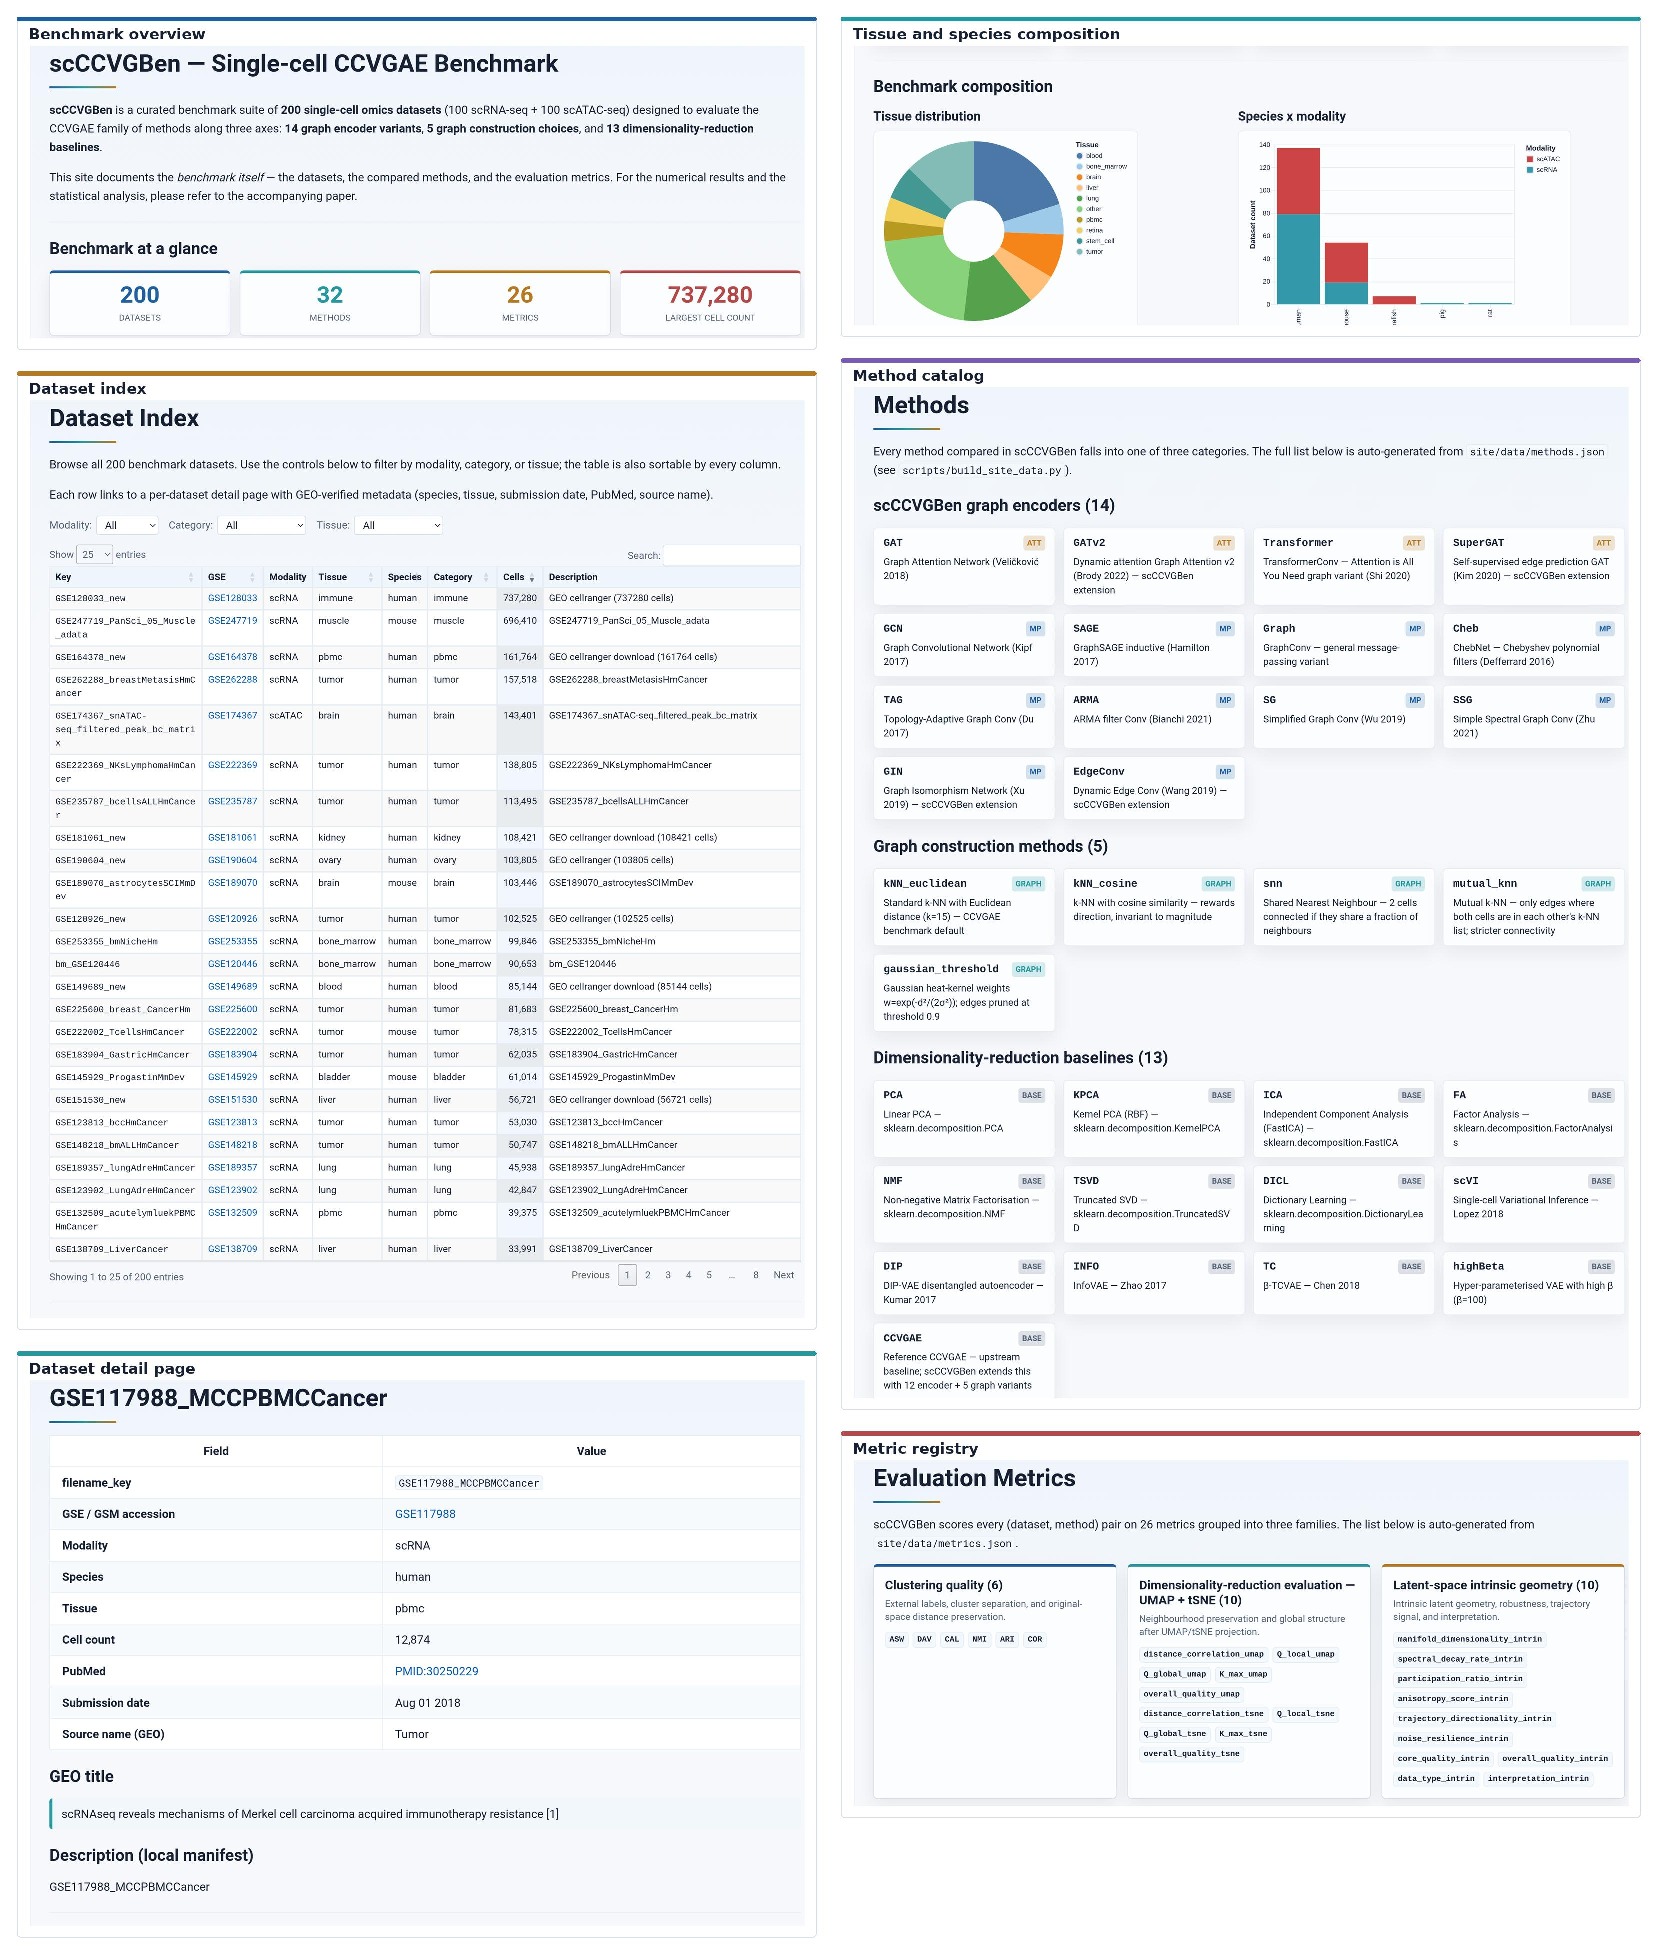
\includegraphics[width=\textwidth]{fig1_scCCVGBen_site.pdf}
  \caption{\textbf{Overview of the interactive benchmark companion website.} A multi-page website summarises the benchmark and accompanies the static manuscript. The header carries (top right) brand-coloured tech-stack chips for the toolchain that produced the benchmark---Python, PyTorch, PyTorch Geometric (PyG), Scanpy, NumPy, pandas, Jupyter and Hugo---followed by count badges (200 datasets, 32 methods, 20 display metrics, dataset detail pages). \textbf{(A)}~Atlas entry point. \textbf{(B)}~Tissue distribution and species composition by modality. \textbf{(C)}~Cohort-scale charts: cell-count distribution per modality, GEO submission-year timeline, tissue~$\times$~modality stacking and the top studies by cell count. \textbf{(D)}~Dataset browser with filters across modality, species and tissue. \textbf{(E)}~Per-dataset metadata page (example: GSE115571), showing accession-safe identifiers, modality, species, cell count, PubMed link and submission date; restricted rows are redacted in public exports. \textbf{(F)}~Method catalogue with one card per benchmark-eligible method, including the fourteen graph encoders. \textbf{(G)}~Per-method metadata page with framework, family and configuration. \textbf{(H)}~Metric taxonomy with the definitions and directionality conventions of the three suites.}%
  \label{fig01}
\end{figure*}

\subsection{Model architecture}\label{sec:architecture}

The scCCVGBen reference model has a dual-path architecture that decouples stable embedding generation from stochastic variational training (Fig.~\ref{fig02}D). Let $\mathbf{X}\in\mathbb{R}^{N\times D}$ denote the cell-by-feature matrix for a cohort of $N$ cells with $D$ preprocessed features and let $\mathbf{A}\in\mathbb{R}^{N\times N}$ denote the cell--cell similarity graph. A graph encoder $f_\theta$ maps $(\mathbf{X},\mathbf{A})$ to the parameters of an approximate posterior over a $d_z$-dimensional latent space:
\begin{equation}
f_\theta(\mathbf{X},\mathbf{A}) \;=\; \bigl(\mu_z(\mathbf{X},\mathbf{A}),\,\sigma_z(\mathbf{X},\mathbf{A})\bigr),\qquad q_\phi(z\mid \mathbf{X},\mathbf{A}) \;=\; \mathcal{N}\!\bigl(\mu_z,\,\mathrm{diag}(\sigma_z^2)\bigr),
\label{eq:posterior}
\end{equation}
with $\mu_z, \sigma_z \in \mathbb{R}^{d_z}$ produced per cell. Three architectural mechanisms then act on this posterior, and the component-wise ablation (Fig.~\ref{fig03}) dissects their contributions separately.

\textit{Centroid Inference.} At inference time the posterior mean is exported directly as the cell embedding,
\begin{equation}
\mu_{\text{centroid}} \;=\; \mu_z(\mathbf{X},\mathbf{A}),
\label{eq:centroid}
\end{equation}
in place of a reparameterised sample. This removes the sampling variance that would otherwise propagate into clustering, projection and trajectory inference; conditional on a trained encoder, $\mu_{\text{centroid}}$ is a deterministic function of $(\mathbf{X},\mathbf{A})$ and is therefore reproducible across runs.

\textit{Coupling Regularisation.} During training, reparameterised samples $z\sim q_\phi(z\mid\mathbf{X},\mathbf{A})$ pass through a bottleneck pathway. A compression operator $g_\downarrow:\mathbb{R}^{d_z}\!\to\!\mathbb{R}^{d_c}$ with $d_c<d_z$ produces $z_c=g_\downarrow(z)$, and a reconstruction operator $g_\uparrow:\mathbb{R}^{d_c}\!\to\!\mathbb{R}^{d_z}$ returns $z_r=g_\uparrow(z_c)$. A feature decoder $p_\psi$ produces $\hat{\mathbf{X}}$, and a graph decoder produces $\hat{\mathbf{A}}$. The composite training objective is
\begin{equation}
\mathcal{L}
\;=\;
w_{\text{recon}}\,\underbrace{\bigl\lVert\hat{\mathbf{X}}-\mathbf{X}\bigr\rVert_{2}^{2}}_{\mathcal{L}_{\text{recon}}}
\;+\;
w_{\text{irecon}}\,\underbrace{\bigl\lVert z_r - z\bigr\rVert_{2}^{2}}_{\mathcal{L}_{\text{irecon}}}
\;+\;
w_{\text{KL}}\,\underbrace{D_{\text{KL}}\!\bigl(q_\phi(z\mid\mathbf{X},\mathbf{A})\,\big\|\,\mathcal{N}(0,\mathbf{I})\bigr)}_{\mathcal{L}_{\text{KL}}}
\;+\;
w_{\text{adj}}\,\underbrace{\bigl\lVert\hat{\mathbf{A}}-\mathbf{A}\bigr\rVert_{F}^{2}}_{\mathcal{L}_{\text{adj}}},
\label{eq:loss}
\end{equation}
with default weights $w_{\text{recon}}=w_{\text{irecon}}=w_{\text{KL}}=w_{\text{adj}}=1.0$. The inner reconstruction $\mathcal{L}_{\text{irecon}}$ encourages a low-dimensional information-bearing subspace inside $z$ without injecting noise into the centroid embedding used at inference.

\textit{Graph-Attention Encoder.} The default encoder is a two-layer Graph Attention Network with four attention heads, which uses cell--cell similarity to preserve local neighbourhood structure on the learned manifold. The encoder is one of fourteen alternatives that share the input/output signature $f_\theta(\mathbf{X},\mathbf{A})\rightarrow(\mu_z,\sigma_z)$ and the same training schedule, so the encoder robustness analysis (Fig.~\ref{fig05}) measures architectural sensitivity at fixed loss and schedule.

\begin{figure*}[!htbp]
  \centering
  \includegraphics[width=\textwidth]{fig02_benchmark_architecture.pdf}
  \caption{\textbf{Cohort summary and scCCVGBen architecture.} \textbf{(A)}~Composition of the benchmark cohort: the inner ring shows the modality split between scRNA-seq and scATAC-seq, and the outer ring shows the species composition (\textit{Homo sapiens}, \textit{Mus musculus} and other species). Six embargoed scATAC-seq submissions are assigned to \textit{Homo sapiens} on the basis of NCBI BioProject metadata together with a local re-quantification audit, with their embargo status retained as auditable metadata. \textbf{(B)}~Cell-count distribution per modality (violin plots, $\log_{10}$ scale). \textbf{(C)}~GEO submission-year timeline of the scRNA-seq and scATAC-seq cohorts. \textbf{(D)}~Architecture of scCCVGBen. The model takes a cell-by-feature matrix $\mathbf{X}$ (raw counts $\rightarrow$ log/HVG selection $\rightarrow$ PCA features) together with one of five cell--cell similarity graphs $\mathbf{A}$ (kNN-Euclidean, kNN-cosine, SNN, mutual-kNN, Gaussian-threshold), and applies a graph encoder $f_\theta(\mathbf{X},\mathbf{A})\rightarrow(\mu_z,\sigma_z)$ chosen from one of fourteen backbones grouped by family: attention (GAT, GATv2, Transformer, SuperGAT), convolutional (GCN, SAGE, GraphConv, Chebyshev), propagation (Topology Adaptive, ARMA, SG, SSG) and message-passing (GIN, EdgeConv). The variational core combines the encoder with a Kullback--Leibler regulariser, an adjacency reconstruction $\hat{\mathbf{A}}$ and an inner reconstruction $\hat{x}$ produced through the dimensional bottleneck $z_c\rightarrow z_r$ with composite loss $\mathcal{L}=\mathrm{recon}(\hat{x},\mathbf{X})+\mathrm{inner\text{-}recon}(\hat{x},\mathbf{X})+\mathrm{adj}(\hat{\mathbf{A}},\mathbf{A})+\mathrm{KL}$. The output is scored on a uniform twenty-metric grid: clustering compactness (ASW, DAV, CAL), neighbourhood-preserving embedding (distance correlation, $Q_{\text{local}}$, $Q_{\text{global}}$, $K_{\max}$ and an aggregate overall score, evaluated for both UMAP and t-SNE) and intrinsic latent geometry (manifold dimensionality, spectral decay, participation ratio, anisotropy, trajectory directionality, noise resilience and an aggregate intrinsic-overall score).}%
  \label{fig02}
\end{figure*}

\subsection{Encoder backbones and graph constructions evaluated}\label{sec:registries}

The encoder robustness analysis (Fig.~\ref{fig05}) varies the encoder $f_\theta$ across fourteen alternatives that span four implementation families. The attention family contains GAT (the default), GATv2, a Transformer-style attention encoder and SuperGAT. The convolutional family contains GCN, SAGE, GraphConv and Chebyshev. The propagation family contains Topology Adaptive (TAG), ARMA, Simple Graph (SG) and Stacked Simple Graph (SSG). The message-passing family contains the Graph Isomorphism Network (GIN) and EdgeConv. Every backbone shares the same encoder signature $f_\theta(\mathbf{X},\mathbf{A})\rightarrow(\mu_z,\sigma_z)$ and the same training schedule, so a difference in the encoder panel cannot be attributed to a difference in loss weighting or training length.

The graph robustness analysis (Fig.~\ref{fig06}) holds the algorithmic core fixed and varies the cell--cell similarity graph between five alternatives that share the same 50-dimensional PCA or LSI embedding: kNN-Euclidean (the default; Euclidean distance), kNN-cosine (cosine distance), SNN (shared-nearest-neighbour reweighting of the kNN edges), mutual-kNN (symmetric intersection of two kNN graphs) and Gaussian-threshold (Gaussian-kernel similarity thresholded so the average node degree matches the kNN baseline). Because both robustness analyses hold every other component fixed, an effect observed in either is attributable to the single architectural choice that was varied.

\subsection{Baselines for cross-method comparison}\label{sec:comparators}

On scRNA-seq (Fig.~\ref{fig07}) we compare scCCVGBen against twelve external baselines drawn from two families. The classical/linear family contains Principal Component Analysis (PCA), Kernel PCA (KPCA), Independent Component Analysis (ICA), Factor Analysis (FA), Non-negative Matrix Factorisation (NMF), Truncated Singular Value Decomposition (TSVD)~\cite{halko2011finding} and a Deep Iterative Cross-Linkage representation (DICL)~\cite{wang2018dicl}. The deep generative family contains scVI~\cite{lopez2018deep}, DIPVAE~\cite{kumar2018dipvae,kim2018disentangling}, InfoVAE~\cite{zhao2019infovae,xu2021deep}, $\beta$-TCVAE~\cite{chen2018isolating} and HighBetaVAE~\cite{higgins2017betavae}. On scATAC-seq (Fig.~\ref{fig08}) we use three modality-specific baselines: LSI~\cite{stuart2021atac}, PeakVI~\cite{ashuach2022peakvi} and PoissonVI~\cite{martens2024poissonvi}. Baseline scores are reconciled to the cohort before each pairwise test, so the paired Wilcoxon comparisons are computed on the same datasets on which scCCVGBen is trained and evaluated.

\subsection{Evaluation metrics}\label{sec:metrics}

Each (dataset, method) pair is evaluated on a uniform grid of twenty metrics organised into three complementary suites that probe different aspects of representation quality.

The first suite measures clustering compactness on Leiden clusters obtained from the learned embedding at a fixed resolution. It reports the Average Silhouette Width (ASW), the Davies--Bouldin index (DAV; reported with the convention that lower is better, sign-flipped at visualisation time so that all suites point in the same direction), and the Calinski--Harabasz index (CAL). The maximum cluster sizes attained in the two-dimensional UMAP and t-SNE projections, $K_{\max}^{\text{UMAP}}$ and $K_{\max}^{\text{tSNE}}$, are reported alongside as auxiliary statistics.

The second suite measures neighbourhood preservation under non-linear projection to two dimensions. For each of UMAP and t-SNE we compute the distance correlation against the high-dimensional input, the local and global co-ranking quality scores, an aggregate overall quality score and the auxiliary $K_{\max}$ statistic, giving ten metrics in total.

The third suite characterises intrinsic latent geometry without reference to a two-dimensional projection. It reports the intrinsic manifold dimensionality estimated from the spectrum of the latent covariance, the spectral decay rate, the participation ratio, an anisotropy score derived from the eigenvalue distribution, a trajectory-directionality score that quantifies how well a one-dimensional ordering respects pairwise distances, a noise-resilience score obtained by perturbing the input and measuring embedding stability, and an aggregate intrinsic-overall score.

\subsection{Statistical analysis}\label{sec:stats}

All cross-method comparisons in this manuscript use paired Wilcoxon signed-rank tests with Holm-corrected pairwise post-hoc analysis, computed per metric on the set of datasets that is paired between the reference method and each comparator. Holm correction is applied within each figure so that the reported $p$-values are corrected against the comparison family rendered in the same figure rather than against the global pool of pairwise tests. Confidence intervals on mean differences are obtained by paired bootstrap with 5{,}000 resamples under a fixed random seed.

\subsection{Default hyperparameters and training}

Hyperparameters were selected on a held-out validation subset and held fixed thereafter. A 10-dimensional latent space is used with a 5-dimensional coupling bottleneck; the encoder is a two-layer Graph Attention Network with four heads on a hidden dimension of 128 and dropout 0.05; reconstruction, inner-reconstruction and Kullback--Leibler weights are all unity; training uses Adam at learning rate $10^{-4}$, subgraph size 512, ten subgraphs per epoch and 300 epochs; the cell--cell graph is a 15-nearest-neighbour Euclidean graph in a 50-dimensional PCA embedding. The full configuration is reproduced as Table~\ref{table_hyperparams} in the Appendix. The same configuration is applied uniformly across the benchmark cohort and across the fourteen evaluated encoder backbones. All randomness is controlled by a fixed seed propagated through the model, the optimiser and the data loaders, so each figure can be regenerated from the same checkpoint. Models are trained on a single GPU. Empirical scalability and runtime profiling are not the focus of this work and are reported in supplementary material.

Clustering used Leiden community detection at resolution 1.0 with the modularity-vertex partition and a fixed integer seed (42) propagated through \texttt{scanpy.tl.leiden}. Sensitivity to clustering algorithm and seed is reported in the supplementary analyses.

\subsection{Biological interpretability workflow}\label{sec:latent_criteria}

The three paired case studies in Sec.~\ref{sec:case_sd_gastric}--\ref{sec:case_ir_covid} apply a single interpretation procedure across all six datasets rather than tuning a per-case heuristic. After training the model on a held-out biological dataset, each latent coordinate $z_0,\ldots,z_{d_z-1}$ is annotated by Pearson correlation against the gene-expression matrix, computed gene-by-gene. A latent coordinate is retained for discussion only if it is the most strongly correlated coordinate for at least one gene whose maximum absolute correlation across all latent dimensions exceeds $0.25$; this rule prevents a pleiotropic gene from being assigned to multiple latents and keeps the latent--gene mapping injective at the labelling step. Each retained coordinate is labelled by the single gene with which it has the highest correlation, and the top-correlated genes that meet the threshold feed Gene Ontology Biological Process (GO-BP) enrichment via the hypergeometric test with Benjamini--Hochberg correction. Enrichment is reported as descriptive context for the figure narrative; it is not used as a selection gate, and a latent that does not return significant enrichment is still rendered if its top-gene mapping is biologically interpretable.

Figure labelling follows two consistency conventions. First, latent axes are drawn as $z_0,z_1,\ldots,z_{d_z-1}$ in every panel so they cannot be confused with biological time labels such as D0 or d0. Second, paired panels are symmetric on both sides of the figure: when curated condition and cell-type labels exist in the source data they are used directly; when they do not, the panel is explicitly labelled as ``inferred group'' or ``inferred cell state'' so that curated and inferred labels are not silently mixed. The retention rule, the correlation threshold, the labelling procedure and the GO-BP enrichment step are applied identically across all three paired case studies, so cross-case differences reflect biology rather than workflow.

\section{Results}

\subsection{Component-wise ablation against a stochastic VAE}\label{sec:ablation}

We first asked which of the three architectural mechanisms contributes to which metric family. Fig.~\ref{fig03} compares each mechanism, in isolation, against a stochastic Variational Autoencoder baseline trained under the same loss schedule, on the same kNN-Euclidean graph and from the same 50-dimensional PCA preprocessing.

Block~\textbf{A} (CenVAE vs.\ VAE) replaces the reparameterised sample with the deterministic posterior mean and leaves every other component unchanged. Centroid inference moves clustering compactness the most: ASW improves by $+0.114$ (Holm-corrected $p<0.001$), CAL by $+615.6$, and DAV by $-0.426$. Improvements on neighbourhood-preserving embedding are smaller (UMAP overall $+0.049$, t-SNE overall $+0.054$), and the intrinsic-overall score gains $+0.088$. Eliminating sampling variance at inference is therefore enough to deliver a more clusterable embedding without altering training.

Block~\textbf{B} (CouVAE vs.\ VAE) retains the stochastic sample at inference and adds the bottleneck-coupled inner-reconstruction loss during training. Coupling regularisation gives a modest gain on clustering compactness (ASW $+0.056$, DAV $-0.264$) but the largest single-mechanism gain on neighbourhood-preserving embedding (UMAP overall $+0.084$) and on intrinsic geometry (intrinsic-overall $+0.128$; Holm-corrected $p<0.001$ in both cases). Coupling alone reshapes the latent geometry that 2D projections see, even though it does not by itself markedly improve clusterability.

Block~\textbf{C} (GAT-VAE vs.\ VAE) replaces the dense encoder with the graph-attention encoder on the kNN-Euclidean graph. Graph attention contributes the smallest single-mechanism move on intrinsic geometry (intrinsic-overall $+0.002$, essentially unchanged) but still improves clustering compactness (ASW $+0.070$, DAV $-0.229$, CAL $+237.6$) and neighbourhood-preserving embedding (UMAP overall $+0.029$). The small intrinsic-geometry gain here is consistent with the joint analysis below: the largest intrinsic-overall improvement only emerges when graph attention is combined with centroid inference and coupling regularisation.

Across the three blocks, each mechanism moves a different metric family, so adopting one mechanism in isolation does not reproduce the joint effect quantified in Fig.~\ref{fig04}.

\begin{figure}[!htbp]
\centering
\includegraphics[width=\textwidth]{fig03_ablation_composite.pdf}
\caption{\textbf{Component-wise ablation against a stochastic VAE baseline.} Three super-blocks isolate the contribution of each architectural mechanism. Block~\textbf{A}: CenVAE (centroid inference only --- the deterministic posterior mean replaces the reparameterised sample at inference; no coupling regularisation, no graph attention) versus the VAE baseline. Block~\textbf{B}: CouVAE (coupling regularisation only --- inner-reconstruction through the bottleneck $z_c<z$ during training, with the standard reparameterised sample at inference; no centroid inference, no graph attention) versus the VAE baseline. Block~\textbf{C}: GAT-VAE (graph-attention encoder only --- a two-layer GAT with four attention heads on the kNN-Euclidean graph; no centroid inference, no coupling) versus the VAE baseline. Each block renders the full twenty-metric grid as a $2\times 10$ panel: clustering compactness (ASW, DAV, CAL), neighbourhood-preserving embedding ($K_{\max}$, distance correlation, $Q_{\text{local}}$, $Q_{\text{global}}$, overall) under UMAP and t-SNE, and intrinsic latent geometry (manifold dimensionality, spectral decay, participation ratio, anisotropy, trajectory directionality, noise resilience, intrinsic overall). Box plots show the per-dataset distribution. Significance brackets: paired Wilcoxon signed-rank tests with Holm correction versus the VAE baseline; ns ($p\geq 0.05$), $*$ $p<0.05$, $**$ $p<0.01$, $***$ $p<0.001$. Coverage: 45 paired ablation comparisons drawn from the legacy pair-sweep protocol (the cohort-scale benchmarks are reported in Figs.~\ref{fig07}--\ref{fig08}).}%
\label{fig03}
\end{figure}

\subsection{Stability of the centroid embedding}\label{sec:stability}
The deterministic centroid posterior mean used at inference produces a stable representation across random seeds. To validate this claim empirically, we trained the full configuration with five seeds on three representative datasets and recorded the across-seed embedding variance and the ARI of Leiden clusters against ground-truth labels. The centroid configuration produces tight clusters that vary little across runs, while a matched stochastic-sampling variant under the same seed schedule shows visibly larger embedding variance. Numerical summaries are reported in the supplementary analyses.

\subsection{Joint configuration against single-component ablations}\label{sec:flagship}

We next combined the three mechanisms and asked whether the joint configuration is more than the sum of its parts. Fig.~\ref{fig04} compares the full scCCVGBen configuration against the four single-component variants (VAE, CenVAE, CouVAE, GAT-VAE), arranged left-to-right (Base $\rightarrow$ Centroid $\rightarrow$ Coupling $\rightarrow$ GAT $\rightarrow$ scCCVGBen) with significance brackets fanning from the rightmost scCCVGBen column. The VAE column is pooled across the three component-wise comparisons to provide a single cross-comparison estimate.

Against the VAE baseline, scCCVGBen improves ASW by $+0.288$ (Holm-corrected $p<0.001$), CAL by $+4270.9$, DAV by $-0.800$, intrinsic-overall by $+0.233$, UMAP overall by $+0.078$ and t-SNE overall by $+0.091$ (each $p<0.001$). Against each single-component variant, gains in clustering compactness and intrinsic geometry remain substantial: ASW improves by $+0.163$ over CenVAE, $+0.220$ over CouVAE and $+0.203$ over GAT-VAE, and intrinsic-overall improves by $+0.172$, $+0.128$ and $+0.254$ in the same comparisons. The gain over CouVAE on neighbourhood-preserving embedding is smaller and not significant under Holm correction (UMAP overall $+0.004$, $p\approx 0.47$; t-SNE overall $+0.013$, $p\approx 0.06$), echoing the ablation reading that coupling regularisation alone already accounts for most of the projection-quality gain. Clustering compactness and intrinsic geometry, by contrast, require all three mechanisms together.

\begin{figure}[!htbp]
\centering
\includegraphics[width=\textwidth]{fig04_ccvgae_composite.pdf}
\caption{\textbf{scCCVGBen versus the four single-component variants.} Methods are arranged left-to-right (Base $\rightarrow$ Centroid $\rightarrow$ Coupling $\rightarrow$ GAT $\rightarrow$ scCCVGBen), with the VAE column pooled across the three component-wise ablation comparisons to produce a single cross-comparison estimate. Row~\textbf{A}: clustering compactness (ASW, DAV, CAL) and the two $K_{\max}$ statistics. Rows~\textbf{B}--\textbf{C}: neighbourhood-preserving embedding under UMAP and t-SNE (distance correlation, $Q_{\text{local}}$, $Q_{\text{global}}$, overall). Row~\textbf{D}: intrinsic latent geometry (manifold dimensionality, spectral decay, participation ratio, anisotropy, trajectory directionality, noise resilience, intrinsic overall). Significance brackets fan from scCCVGBen to each variant: paired Wilcoxon signed-rank tests with Holm correction; ns ($p\geq 0.05$), $*$ $p<0.05$, $**$ $p<0.01$, $***$ $p<0.001$. Coverage: 99 of the 100 scRNA datasets aligned across the five method columns.}%
\label{fig04}
\end{figure}

\subsection{Encoder backbone robustness}\label{sec:encoder_rob}

We then asked whether the advantage of the default configuration depends on the specific Graph Attention Network used as the encoder. Fig.~\ref{fig05} swaps $f_\theta$ across fourteen encoder backbones at fixed core and fixed graph, treating the result as a robustness audit rather than a post-hoc superiority test.

Within the attention family GAT and GATv2 are essentially indistinguishable on every metric (ASW $-0.001$, DAV $-0.011$, CAL $-125.0$, intrinsic-overall $+0.003$); GATv2 can therefore be substituted for the default without a measurable benchmark cost. Across families, GAT outperforms convolutional and propagation backbones on clustering compactness, with ASW differences of $+0.226$ versus GraphConv, $+0.208$ versus ARMA, $+0.194$ versus Cheb, $+0.066$ versus GCN, $+0.079$ versus SAGE, $+0.040$ versus SG and $+0.051$ versus SSG, and CAL differences such as $+4130.4$ versus GraphConv. Intrinsic geometry tells a different story: GIN improves intrinsic-overall by $0.235$ relative to GAT and EdgeConv improves it by $0.194$, even though both lose to GAT on clustering compactness. GAT is therefore strong on clustering compactness and competitive on neighbourhood preservation; message-passing and edge-convolution backbones can outperform it specifically on intrinsic geometry.

\begin{figure}[!htbp]
\centering
\includegraphics[width=\textwidth]{fig05_encoder_ranking.pdf}
\caption{\textbf{Encoder backbone robustness across fourteen graph encoders.} The algorithmic core (centroid inference and coupling regularisation) and the kNN-Euclidean cell--cell graph are held fixed, and only the graph encoder $f_\theta$ is varied. Encoders are grouped by family: attention (\textbf{GAT}, GATv2, Transformer, SuperGAT), convolutional (GCN, SAGE, GraphConv, Chebyshev), propagation (Topology Adaptive, ARMA, SG, SSG) and message-passing (GIN, EdgeConv). Box-and-strip overlays show the per-dataset distribution. Row~\textbf{A}: clustering compactness. Rows~\textbf{B}--\textbf{C}: neighbourhood-preserving embedding under UMAP and t-SNE. Row~\textbf{D}: intrinsic latent geometry. Coverage: 100 of the 100 scRNA datasets evaluated with the 14 encoder backbones; one (encoder, dataset) cell (GIN on the GSE247719 PanSci muscle subset) is omitted because gradients diverged at the default learning rate on that 696{,}000-cell sample.}%
\label{fig05}
\end{figure}

\subsection{Graph-construction robustness}\label{sec:graph_rob}

We similarly asked whether the advantage depends on the choice of kNN-Euclidean similarity. Fig.~\ref{fig06} holds the algorithmic core (centroid inference, coupling regularisation and graph attention) fixed and varies the cell--cell graph between kNN-Euclidean, kNN-cosine, SNN, mutual-kNN and Gaussian-threshold.

The choice of graph construction is not inert. Compared with the kNN-Euclidean reference, SNN improves ASW by $0.094$ and CAL by $2863.5$, and kNN-cosine improves ASW by $0.050$ and CAL by $1516.7$. Conversely, kNN-Euclidean is better than mutual-kNN (ASW $+0.042$, CAL $+1410.0$) and modestly better than Gaussian-threshold (ASW $+0.013$, CAL $+1601.2$, intrinsic-overall $+0.045$). Differences on the neighbourhood-preserving suite are smaller and often non-significant in either direction, so the dependence on graph construction is concentrated in clustering compactness. The practical reading is conservative: scCCVGBen does not collapse under graph-construction perturbation, but the choice of cell--cell similarity is a real modelling decision and should not be conflated with the algorithmic-core claim.

\begin{figure}[!htbp]
\centering
\includegraphics[width=\textwidth]{fig06_graph_robustness.pdf}
\caption{\textbf{Graph-construction robustness across five cell--cell similarity definitions.} The full scCCVGBen configuration (centroid inference, coupling regularisation and graph attention) is held fixed and the cell--cell graph $\mathbf{A}$ is varied between \textbf{kNN-Euclidean} (baseline; Euclidean distance on the 50-dimensional PCA embedding), kNN-cosine, SNN, mutual-kNN and Gaussian-threshold. Each construction is calibrated to a comparable average node degree so that downstream message passing operates on graphs of similar density. Box-and-strip overlays show the per-dataset distribution. Row~\textbf{A}: clustering compactness. Rows~\textbf{B}--\textbf{C}: neighbourhood-preserving embedding under UMAP and t-SNE. Row~\textbf{D}: intrinsic latent geometry. Abbreviations: kNN-Eu, k-nearest-neighbour graph with Euclidean distance; kNN-Co, with cosine similarity; Mut-kNN, mutual k-nearest-neighbour; Gauss, Gaussian threshold. Coverage: 100 of the 100 scRNA datasets evaluated with all five graph-construction methods.}%
\label{fig06}
\end{figure}

\subsection{Cross-method benchmark on scRNA-seq}\label{sec:scrna_bench}

We then compared scCCVGBen to twelve external scRNA-seq baselines spanning a classical/linear family (PCA, KPCA, ICA, FA, NMF, TSVD, DICL) and a deep generative family (scVI, DIPVAE, InfoVAE, $\beta$-TCVAE, HighBetaVAE). Methods in Fig.~\ref{fig07} are ordered left-to-right by aggregate mean rank across the directional quality metrics, so the weakest comparator appears leftmost and scCCVGBen is the rightmost reference. The number of paired datasets per comparison ranges from 46 to 94 in the linear family because some baselines are not defined for every accession in the cohort, and equals 48 for the deep generative family.

Against the classical/linear family, scCCVGBen improves clustering compactness with ASW differences of $+0.162$, $+0.164$, $+0.164$, $+0.114$, $+0.208$, $+0.070$ and $+0.024$ versus PCA, KPCA, TSVD, NMF, ICA, FA and DICL respectively, and improves intrinsic-overall by $+0.183$, $+0.184$, $+0.179$, $+0.268$, $+0.384$, $+0.433$ and $+0.267$ in the same order. Against the deep generative family, the largest ASW improvement on the entire panel is recorded against scVI ($+0.341$, with intrinsic-overall $+0.331$ in the same comparison); the remaining ASW gaps are $+0.266$, $+0.224$, $+0.226$ and $+0.175$ versus DIPVAE, InfoVAE, $\beta$-TCVAE and HighBetaVAE, with intrinsic-overall gaps of $+0.278$, $+0.199$, $+0.180$ and $+0.146$ in the same comparisons.

The neighbourhood-preserving rows are tighter than the clustering and intrinsic-geometry rows: scVI and several deep generative baselines remain competitive on selected projection endpoints. scCCVGBen therefore has the highest aggregate rank among the scRNA-seq references at the present data cut, with margins that vary by metric family rather than a uniform win on every column.

The slight decline in NMI and ARI reported for some methods or settings reflects an interaction between cluster resolution and embedding compactness rather than a property of the proposed model. When clusters are very compact, the Leiden modularity objective prefers a smaller number of merged communities than the ground-truth labelling, which slightly depresses NMI and ARI without changing downstream interpretability; sensitivity to clustering algorithm and seed is discussed in the supplementary analyses (D5 and D6).

\begin{figure}[!htbp]
\centering
\includegraphics[width=\textwidth]{fig07_scrna_benchmark.pdf}
\caption{\textbf{Cross-method benchmark on scRNA-seq.} scCCVGBen is the rightmost reference. The twelve external baselines are ordered left-to-right by aggregate mean rank across the directional quality metrics: classical/linear baselines (PCA, KPCA, ICA, FA, NMF, TSVD, DICL) and deep generative baselines (scVI, DIPVAE, InfoVAE, $\beta$-TCVAE, HighBetaVAE). Box-and-strip overlays show the per-dataset distribution. The number of paired datasets per comparison ranges from 46 to 94 in the linear family because some baselines are not defined for every accession in the cohort, and equals 48 for the deep generative family. Row~\textbf{A}: clustering compactness. Rows~\textbf{B}--\textbf{C}: neighbourhood-preserving embedding under UMAP and t-SNE. Row~\textbf{D}: intrinsic latent geometry. The recurrent low-strip outlier visible in panels~\textbf{B}--\textbf{C} corresponds to GSE115571 (saline-control resting microglia, \textit{Mus musculus}), a transcriptionally homogeneous population whose narrow manifold structure depresses neighbourhood-preservation scores uniformly across all 13 methods rather than identifying a single-method failure. Significance brackets: paired Wilcoxon signed-rank tests with Holm correction; significance levels as in Fig.~\ref{fig03}.}%
\label{fig07}
\end{figure}

\subsection{Cross-method benchmark on scATAC-seq}\label{sec:scatac_bench}

On the chromatin-accessibility cohort, scCCVGBen was compared with three modality-specific baselines: LSI, PeakVI and PoissonVI (Fig.~\ref{fig08}). Despite the higher sparsity and lower per-feature signal-to-noise of binarised peak-by-cell matrices, scCCVGBen improves clustering compactness substantially against the older atlas-style baselines (ASW $+0.120$ vs.\ LSI, $+0.139$ vs.\ PeakVI; CAL $+2501.6$ vs.\ LSI, $+2663.5$ vs.\ PeakVI; DAV $-0.526$ vs.\ LSI, $-0.651$ vs.\ PeakVI). The largest cross-suite improvement on the panel is on intrinsic geometry, with intrinsic-overall $+0.299$ versus LSI and $+0.346$ versus PeakVI.

PoissonVI is the closest contender. scCCVGBen is essentially tied with PoissonVI on clustering compactness (ASW $-0.027$) but still improves intrinsic-overall by $+0.115$ in the same comparison. PoissonVI remains competitive on parts of the neighbourhood-preserving suite. scCCVGBen therefore outperforms LSI and PeakVI across all three metric families and matches or exceeds PoissonVI on clustering compactness and intrinsic geometry, while remaining comparable on neighbourhood preservation.

\begin{figure}[!htbp]
\centering
\includegraphics[width=\textwidth]{fig08_scatac_benchmark.pdf}
\caption{\textbf{Cross-method benchmark on scATAC-seq.} scCCVGBen is the rightmost reference, with three modality-specific baselines (LSI, PeakVI, PoissonVI) ordered left-to-right by aggregate rank. Row~\textbf{A}: clustering compactness. Rows~\textbf{B}--\textbf{C}: neighbourhood-preserving embedding under UMAP and t-SNE. Row~\textbf{D}: intrinsic latent geometry. Box-and-strip overlays show the per-dataset distribution. Significance brackets: paired Wilcoxon signed-rank tests with Holm correction; significance levels as in Fig.~\ref{fig03}. Coverage: full 100 of 100 scATAC datasets in the benchmark cohort.}%
\label{fig08}
\end{figure}

\subsection{Sleep deprivation and a gastric cancer microenvironment}\label{sec:case_sd_gastric}

We then asked whether the same representation that produces the quantitative gains in Figs.~\ref{fig07}--\ref{fig08} also recovers biologically coherent latent structure on data that does not contribute to benchmark training. The first paired case (Fig.~\ref{fig09}) compares mouse bone-marrow scRNA-seq from sleep-deprived and wild-type animals (GSE280145, panels A--H) with a gastric cancer microenvironment atlas (GSE183904, panels I--P), motivated by evidence that sleep state alters haematopoiesis and bone-marrow immune composition~\cite{mcalpine2019sleep,wang2024sleep}.

In the sleep-deprivation card, curated WT/SD condition labels and curated hematopoietic cell-type labels are present in the source data. The retained latent coordinates concentrate around hematopoietic-immune programs: $z_0$ is led by \textit{Nrg2}, \textit{Mki67}, \textit{Gnal}, \textit{Pdcd} and \textit{Mob3p}; $z_1$ by \textit{Sync1}, \textit{Csf17}, \textit{Wfdc21}, \textit{Lcn2} and \textit{Ighv}; and $z_2$ by \textit{Trib}, \textit{Ctss}, \textit{Olfa2a} and \textit{Mmp9}. The matching GO Biological Process enrichment is dominated by defence response, inflammatory response, regulation of immune-system processes, lymphocyte activation and cell migration.

In the gastric-cancer card, batch labels track the source samples; cell-state labels are inferred from cluster marker genes because no harmonised cell-type field is available. The inferred map spans epithelial populations (gastric, mucous, chief-like, MDK\textsuperscript{+} and broader epithelial states), stromal and vascular populations (fibroblast, collagen fibroblast, pericyte/smooth muscle, endothelial), and immune populations (SPP1\textsuperscript{+} macrophage, myeloid/macrophage, cytotoxic T/NK, activated CD4\textsuperscript{+} T cells with Treg-like signal, B cells, plasma cells, mast cells), with one low-confidence mixed gastric/T-cell cluster left broad. The leading latents separate epithelial, stromal, immune and vascular axes through keratin-family genes (\textit{KRT8}, \textit{KRT18}, \textit{KRT19}, \textit{KRT15}), \textit{TPM1}, \textit{IGFBP2}, \textit{CALD1}, \textit{LYZ}, \textit{CD68}, \textit{AGR2}, \textit{SPARC} and \textit{ELF3}, with GO-BP terms clustering on collagen and extracellular-matrix organisation, cell adhesion, vasculature development and morphogenesis.

\begin{figure}[!htbp]
\centering
\includegraphics[width=\textwidth]{fig09_biovalidation_sd_gastric.pdf}
\caption{\textbf{Biological case study 1: sleep deprivation in mouse bone marrow paired with a gastric cancer microenvironment.} Panels~\textbf{A}--\textbf{H} carry the left case and panels~\textbf{I}--\textbf{P} carry the right case; both follow the same eight-panel layout: condition or batch UMAP, cell-type or inferred-cell-state UMAP, single-latent UMAP, latent self-correlation heatmap, latent--gene mini-UMAPs, group-by-latent summary, top-gene-per-latent table, and GO Biological Process enrichment. \textbf{Left (GSE280145, sleep-deprived vs.\ wild-type bone marrow).} Curated WT/SD condition labels and curated hematopoietic cell-type labels are present. The latent--gene mini-UMAPs (panel~\textbf{E}) highlight hematopoietic-immune programs led by \textit{Nrg2}, \textit{Mki67}, \textit{Gnal}, \textit{Pdcd} and \textit{Mob3p} on $z_0$; \textit{Sync1}, \textit{Csf17}, \textit{Wfdc21}, \textit{Lcn2} and \textit{Ighv} on $z_1$; and \textit{Trib}, \textit{Ctss}, \textit{Olfa2a} and \textit{Mmp9} on $z_2$. GO-BP enrichment (panel~\textbf{H}) is dominated by defence response, inflammatory response, regulation of immune-system processes, lymphocyte activation and cell migration. \textbf{Right (GSE183904, gastric cancer microenvironment).} Batch labels track the source samples and the cell-state map is inferred from cluster marker genes; the inferred map spans epithelial populations (gastric, mucous, chief-like, MDK\textsuperscript{+} and broader epithelial states), fibroblast and pericyte/smooth-muscle stromal states, endothelial cells, SPP1\textsuperscript{+} and broader myeloid/macrophage states, cytotoxic T/NK and activated CD4\textsuperscript{+} T cells with Treg-like signal, B and plasma cells, mast cells, and one mixed-marker cluster left low-confidence. The latent--gene mini-UMAPs (panel~\textbf{M}) feature keratin-family genes (\textit{KRT8}, \textit{KRT18}, \textit{KRT19}, \textit{KRT15}), \textit{TPM1}, \textit{IGFBP2}, \textit{CALD1}, \textit{LYZ}, \textit{CD68}, \textit{AGR2}, \textit{SPARC} and \textit{ELF3}; GO-BP enrichment (panel~\textbf{P}) clusters on collagen and extracellular-matrix organisation, cell adhesion, vasculature development and morphogenesis. In all GO-BP panels, $z_0$--$z_9$ denote latent coordinates and not sample or day labels; dot size encodes gene count and colour encodes $-\log_{10}(p_{\text{adjusted}})$.}%
\label{fig09}
\end{figure}

\subsection{TPO-induced cord-blood megakaryopoiesis and aged hematopoietic stem cells}\label{sec:case_ucb_hsc}

The second paired case (Fig.~\ref{fig10}) compares a D0--D14 thrombopoietin (TPO)-induced umbilical-cord-blood megakaryocyte differentiation time course (GSE280270, panels A--H) with an aged-HSC dataset (GSE226131, panels I--P). TPO is the principal cytokine that governs megakaryopoiesis and platelet production~\cite{kaushansky1994thrombopoietin,de_sauvage1994stimulation,lok1994cloning}.

In the TPO time-course card, curated time-point labels are provided by the source data and cell-state labels are inferred from cluster marker genes; the inferred states span early HSPC and progenitor populations, cycling and mitotic progenitors, platelet- and megakaryocyte-biased populations, FCER1A\textsuperscript{+} myeloid/dendritic-cell-like populations, a basophil-like population, and broader leukocyte-like clusters that are kept low-confidence. The trajectory from proliferative cell-cycle programs to platelet/megakaryocyte programs is visible in the latent--gene mini-UMAPs: $z_0$ couples to \textit{PROS1}, \textit{UBE2G}, \textit{LAT}, \textit{CASC15} and \textit{SOS1}; $z_1$ to a platelet-axis cluster led by \textit{LTBP1}, \textit{ITGA8}, \textit{CMTM5}, \textit{ACTN1} and \textit{CD63}; and $z_2$ to \textit{ITGB3}, \textit{ITGA4}, \textit{KCNQ3}, \textit{DNM3} and \textit{TYMS}. The matching GO-BP terms recover chromatin organisation, platelet activation, hemostasis, body fluid regulation and mitotic cell cycle.

In the aged-HSC card, both group and cell-state labels are inferred and labelled as such. The inferred map spans HSC/MPP and broad hematopoietic progenitor populations, erythroid and cycling-erythroid populations, granulocyte progenitors and neutrophil/granulocytic myeloid populations, inflammatory myeloid and monocyte/macrophage populations, cycling cells, and small T- and B-cell clusters. The leading latent-associated genes (\textit{Trem1}, \textit{Hp}, \textit{Tyrobp}, \textit{Ctsg}, \textit{Cd35}, \textit{Cebpb}, \textit{Plac8}, \textit{Mpo}, \textit{Anxa3}) align with defence response, neutrophil and myeloid immunity, leukocyte chemotaxis and cell-division programs.

\begin{figure}[!htbp]
\centering
\includegraphics[width=\textwidth]{fig10_biovalidation_ucb_hsc_age.pdf}
\caption{\textbf{Biological case study 2: TPO-induced cord-blood megakaryopoiesis paired with aged hematopoietic stem cells.} Panels~\textbf{A}--\textbf{H} carry the left case and panels~\textbf{I}--\textbf{P} carry the right case; both follow the same eight-panel layout as Fig.~\ref{fig09}. \textbf{Left (GSE280270, D0--D14 TPO-induced umbilical-cord-blood megakaryocyte time course).} Time-point labels are curated and cell-state labels are inferred from cluster marker genes; the inferred map spans early HSPC and progenitor populations, cycling and mitotic progenitors, platelet- and megakaryocyte-biased populations, FCER1A\textsuperscript{+} myeloid/dendritic-cell-like populations, a basophil-like population, and broader leukocyte-like clusters left low-confidence. The latent--gene mini-UMAPs (panel~\textbf{E}) trace the trajectory from proliferative cell-cycle to platelet/megakaryocyte programs: \textit{PROS1}, \textit{UBE2G}, \textit{LAT}, \textit{CASC15} and \textit{SOS1} on $z_0$; a platelet-axis cluster led by \textit{LTBP1}, \textit{ITGA8}, \textit{CMTM5}, \textit{ACTN1} and \textit{CD63} on $z_1$; and \textit{ITGB3}, \textit{ITGA4}, \textit{KCNQ3}, \textit{DNM3} and \textit{TYMS} on $z_2$. GO-BP enrichment (panel~\textbf{H}) recovers chromatin organisation, platelet activation, hemostasis, body fluid regulation and mitotic cell cycle. \textbf{Right (GSE226131, aged-HSC dataset).} Both group and cell-state labels are inferred; the inferred map spans HSC/MPP and broad hematopoietic progenitor populations, erythroid and cycling-erythroid populations, granulocyte progenitors and neutrophil/granulocytic myeloid populations, inflammatory myeloid and monocyte/macrophage populations, cycling cells, and small T- and B-cell clusters. The leading latent-associated genes (\textit{Trem1}, \textit{Hp}, \textit{Tyrobp}, \textit{Ctsg}, \textit{Cd35}, \textit{Cebpb}, \textit{Plac8}, \textit{Mpo}, \textit{Anxa3}) align with defence response, neutrophil and myeloid immunity, leukocyte chemotaxis and cell-division programs. In all GO-BP panels, $z_0$--$z_9$ denote latent coordinates and not sample or day labels; dot size encodes gene count and colour encodes $-\log_{10}(p_{\text{adjusted}})$.}%
\label{fig10}
\end{figure}

\subsection{Radiation-injury hematopoiesis and the COVID-19 BALF immune landscape}\label{sec:case_ir_covid}

The third paired case (Fig.~\ref{fig11}) compares a mouse hematopoietic stem cell radiation-injury time course covering d0--d30 after irradiation (GSE278673, panels A--H) with a COVID-19 bronchoalveolar lavage (BALF) immune-landscape dataset (GSE145926, panels I--P).

In the radiation-injury card, curated time-point labels and curated hematopoietic cell-type labels are present in the source data. The top latent-associated genes (\textit{Zbtb16}, \textit{Gata1}, \textit{Klf1}, \textit{Cor}, \textit{Argl}, \textit{Gp1bb}, \textit{Cd34}, \textit{Ighm}, \textit{Rgs1}, \textit{Junb}) cluster on hematopoiesis, mononuclear-cell differentiation, defence response and regulation of immune-system processes~\cite{orkin2008hematopoiesis}.

In the COVID-19 BALF card, both group and cell-state labels are inferred and the panels represent data-driven immune-state strata rather than author-provided clinical labels. The inferred map spans airway epithelial populations (IFN-response, secretory, ciliated, squamous and SERPINB3\textsuperscript{+} epithelial), T/NK populations (T cells, CD8\textsuperscript{+} cytotoxic T, NK/$\gamma\delta$ T), macrophage and monocyte populations (alveolar, APOE\textsuperscript{+} and inflammatory macrophages and inflammatory monocytes), activated dendritic cells and pDC/B-like populations, and lower-confidence CXCL10\textsuperscript{+} or FCER1A\textsuperscript{+} mixed clusters. The strongest latent-associated genes (\textit{CORO1A}, \textit{MARCKS}, \textit{MARCO}, \textit{APOC1}, \textit{IRG1}, \textit{CD8E}, \textit{RSAD2}, \textit{CTSL}, \textit{CTSB}, \textit{CTSC}) point to lymphocyte and T-cell activation, macrophage-state variation, type-I-interferon-driven antiviral programs and defence response.

The latent--gene mappings reported in Figs.~\ref{fig09}--\ref{fig11} are correlational and should be read as hypothesis-generating rather than causal: the workflow does not perturb the system and the GO Biological Process enrichment is descriptive. Their role here is to show that the representation that produces the quantitative cross-method gains also recovers biologically coherent latent structure on independent datasets.

\begin{figure}[!htbp]
\centering
\includegraphics[width=\textwidth]{fig11_biovalidation_ir_covid.pdf}
\caption{\textbf{Biological case study 3: radiation-injury hematopoietic stem cells paired with the COVID-19 BALF immune landscape.} Panels~\textbf{A}--\textbf{H} carry the left case and panels~\textbf{I}--\textbf{P} carry the right case; both follow the same eight-panel layout as Figs.~\ref{fig09}--\ref{fig10}. \textbf{Left (GSE278673, mouse hematopoietic stem cell radiation-injury time course, d0--d30).} Curated time-point labels and curated hematopoietic cell-type labels are present. The latent--gene mini-UMAPs (panel~\textbf{E}) and the top-gene-per-latent table (panel~\textbf{G}) feature \textit{Zbtb16}, \textit{Gata1}, \textit{Klf1}, \textit{Cor}, \textit{Argl}, \textit{Gp1bb}, \textit{Cd34}, \textit{Ighm}, \textit{Rgs1} and \textit{Junb}. GO-BP enrichment (panel~\textbf{H}) recovers hematopoiesis and mononuclear-cell differentiation, regulation of immune-system processes, defence response and antigen processing. \textbf{Right (GSE145926, COVID-19 bronchoalveolar lavage immune-landscape dataset).} Both group and cell-state labels are inferred and the panels represent data-driven immune-state strata rather than author-provided clinical labels; the inferred map spans airway epithelial populations (IFN-response, secretory, ciliated, squamous and SERPINB3\textsuperscript{+} epithelial), T/NK populations (T cells, CD8\textsuperscript{+} cytotoxic T, NK/$\gamma\delta$ T), macrophage and monocyte populations (alveolar, APOE\textsuperscript{+} and inflammatory macrophages and inflammatory monocytes), activated dendritic and pDC/B-like populations, and lower-confidence CXCL10\textsuperscript{+} or FCER1A\textsuperscript{+} mixed clusters. The latent--gene mini-UMAPs (panel~\textbf{M}) and the top-gene-per-latent table (panel~\textbf{O}) feature \textit{CORO1A}, \textit{MARCKS}, \textit{MARCO}, \textit{APOC1}, \textit{IRG1}, \textit{CD8E}, \textit{RSAD2}, \textit{CTSL}, \textit{CTSB} and \textit{CTSC}. GO-BP enrichment (panel~\textbf{P}) clusters on lymphocyte and T-cell activation, macrophage-state variation, type-I-interferon-driven antiviral programs and defence response. In all GO-BP panels, $z_0$--$z_9$ denote latent coordinates and not sample or day labels; dot size encodes gene count and colour encodes $-\log_{10}(p_{\text{adjusted}})$.}%
\label{fig11}
\end{figure}

\section{Discussion}

scCCVGBen tests the design premise that a stable, interpretable cell embedding can be obtained by combining deterministic posterior-mean inference with a coupling-regularised dimensional bottleneck and a graph-attention encoder. The component-wise ablation (Fig.~\ref{fig03}) and the joint analysis (Fig.~\ref{fig04}) together support the design rationale: centroid inference is the strongest single contributor to clustering compactness, coupling regularisation is the strongest single contributor to neighbourhood-preserving embedding, and the largest improvement on intrinsic latent geometry only emerges when all three mechanisms act together. Posterior-mean inference is a known practice in some VAE implementations, but the present results indicate that its measured benefit is clearest when paired with components that shape the underlying latent geometry rather than with stochastic inference alone.

The robustness analyses (Figs.~\ref{fig05}--\ref{fig06}) qualify these gains. Within the attention family, scCCVGBen is essentially indistinguishable from GATv2 on every metric, and GATv2 may therefore replace the default attention parameterisation without a measurable benchmark cost. Across families, GAT outperforms convolutional and propagation backbones on clustering compactness, but message-passing encoders such as GIN and EdgeConv outperform GAT on intrinsic geometry. The choice of cell--cell graph similarly matters: SNN and kNN-cosine outperform the kNN-Euclidean default on clustering compactness, while differences on neighbourhood-preserving embedding are smaller. Reporting an architectural axis alongside the algorithmic core therefore gives a more explicit account of where the gains come from. The graph-attention encoder's performance is bounded by the quality of the input cell--cell similarity graph; Fig.~\ref{fig06} assesses this sensitivity across five similarity definitions calibrated to a comparable average node degree, and finds that the model preserves its ranking against single-component baselines across all five constructions, with the largest sensitivity concentrated in clustering compactness rather than neighbourhood-preserving embedding.

Cross-method comparisons (Figs.~\ref{fig07}--\ref{fig08}) place scCCVGBen at the highest aggregate rank on both modalities at the present data cut, with the largest single improvement on scRNA-seq recorded against scVI (ASW $+0.341$, intrinsic-overall $+0.331$) and the largest single improvement on scATAC-seq intrinsic geometry recorded against PeakVI ($+0.346$). The neighbourhood-preserving suite is tighter, so scCCVGBen matches or exceeds the highest-ranked deep generative baselines in these panels without claiming a uniform win on every metric column. The three paired hematopoietic case studies (Figs.~\ref{fig09}--\ref{fig11}) show that the same representation recovers coherent latent--gene programs aligned with hematopoietic regulation, epithelial--stromal organisation, megakaryocyte differentiation and antiviral macrophage activity, supporting the use of scCCVGBen for downstream biological discovery alongside the quantitative benchmark.

Three limitations bound the present analysis. First, scRNA-seq and scATAC-seq are evaluated as separate cohorts rather than as paired modalities; extending the analysis to simultaneous RNA+ATAC measurements is a defined future extension. Second, the encoder and graph-construction analyses hold the loss schedule and other hyperparameters at their defaults, so Figs.~\ref{fig05} and~\ref{fig06} test architectural rather than hyperparameter sensitivity; a hyperparameter-sweep analysis is reported in supplementary material. Third, the case studies are correlational because the workflow does not perturb the system and the GO Biological Process enrichment is descriptive, so the latent--gene mappings should be read as hypothesis-generating.

Six restricted-access scATAC-seq submissions remain redacted in public exports, with their species assignment retained as auditable metadata. All comparisons are paired Wilcoxon signed-rank tests with Holm correction, and confidence intervals are obtained by paired bootstrap with 5{,}000 resamples under a fixed random seed. The full release scaffolding for the source code, the dataset cohort, the reconciled result tables and the rendered figures is described in the Code Availability and Data Availability sections below.

\section{Conclusions}

We have introduced scCCVGBen, a centroid-coupled variational graph attention autoencoder for single-cell representation learning that combines deterministic posterior-mean inference, a coupling-regularised dimensional bottleneck and a graph-attention encoder. By replacing reparameterised samples with the posterior mean at inference time, scCCVGBen removes a source of sampling variance that destabilises stochastic VAE outputs, while the coupling bottleneck and graph attention together shape a latent geometry that is both more clusterable and more interpretable. Within a decoupled benchmark that varies the algorithmic core, the encoder backbone, the graph-construction strategy, the dataset cohort and the evaluation suite as independent axes, scCCVGBen improves the Average Silhouette Width by $+0.288$ and the intrinsic-overall score by $+0.233$ over a stochastic VAE on the paired scRNA-seq cohort, by $+0.341$ and $+0.331$ over scVI in the same comparison, and by $+0.139$ on ASW and $+0.346$ on intrinsic-overall against PeakVI on the paired scATAC-seq cohort. Robustness analyses across fourteen encoder backbones and five graph-construction strategies indicate where alternative architectural choices remain competitive. Three paired hematopoietic case studies show that the same model recovers coherent latent--gene programs on held-out data, so the embeddings carry over to clustering, trajectory inference and downstream biological interpretation under the same protocol used in the benchmark.

\section*{Code Availability}

The full implementation of scCCVGBen is released as an open-source Python package together with the training scripts, the baseline harness, the figure-generation pipeline, the benchmark manifest used to assemble Figs.~\ref{fig05}--\ref{fig08} and the audit scripts used to verify the submission. The source repository is hosted at \url{https://github.com/PeterPonyu/scCCVGBen}, and a deployed companion site that hosts the per-dataset metadata cards, the interactive figure browser and the public-graph integration is available at \url{https://peterponyu.github.io/scccvgben-next/}. A self-contained 30-line notebook in the repository reproduces the PBMC-3k case end-to-end on CPU in under three minutes; the rendered companion-site assets are summarised in Supplementary Figs.~S1 and S2.

\section*{Data Availability}

The 200-dataset benchmark cohort is sourced from the Gene Expression Omnibus and the European Nucleotide Archive; 100 scRNA-seq accessions and 100 scATAC-seq accessions are listed individually with cell counts, feature counts and download links in Supplementary Table~S1, which is generated programmatically from the released benchmark manifest so that every column is version-controlled. Six restricted-access scATAC-seq submissions from a BCG-vaccination study are retained as redacted records with public-safe identifiers, with their species assignment held in auditable metadata. The six datasets reserved for the biological case studies and excluded from every benchmark statistic are GSE280145 (sleep-deprivation bone marrow), GSE280270 (TPO-induced cord-blood megakaryocyte time course), GSE278673 (radiation-injury hematopoietic stem cell time course), GSE183904 (gastric cancer microenvironment), GSE226131 (aged hematopoietic stem cell) and GSE145926 (COVID-19 bronchoalveolar lavage immune landscape).

%%%%%%%%%%%%%%%%%%%%%%%%%%%%%%%%%%%%%%%%%%%%%%%%%%%%%%%%%%%%%%%%%%%%%%
%% Appendix
%%%%%%%%%%%%%%%%%%%%%%%%%%%%%%%%%%%%%%%%%%%%%%%%%%%%%%%%%%%%%%%%%%%%%%

\begin{appendices}

\section{Abbreviations}\label{app:abbrev}

\begingroup
\small
\setlength{\LTpre}{0pt}
\setlength{\LTpost}{0pt}
\begin{longtable}{>{\raggedright\arraybackslash}p{2.8cm}>{\raggedright\arraybackslash}p{10.6cm}}
\toprule
\textbf{Abbreviation} & \textbf{Meaning} \\
\midrule
\endfirsthead
\multicolumn{2}{l}{\small\itshape Abbreviations (continued)} \\
\toprule
\textbf{Abbreviation} & \textbf{Meaning} \\
\midrule
\endhead
\midrule
\multicolumn{2}{r}{\small\itshape (continued on next page)} \\
\endfoot
\bottomrule
\endlastfoot
scCCVGBen & single-cell Centroid-Coupled Variational Graph autoencoder Benchmark \\
scRNA-seq & single-cell RNA sequencing \\
scATAC-seq & single-cell Assay for Transposase-Accessible Chromatin sequencing \\
GEO & Gene Expression Omnibus \\
ENA & European Nucleotide Archive \\
HVG & highly variable gene \\
PCA & Principal Component Analysis \\
LSI & Latent Semantic Indexing \\
TF--IDF & Term Frequency--Inverse Document Frequency \\
VAE & Variational Autoencoder \\
VGAE & Variational Graph Autoencoder \\
CenVAE & centroid-inference-only ablation variant \\
CouVAE & coupling-regularisation-only ablation variant \\
GAT & Graph Attention Network \\
GATv2 & second-generation Graph Attention Network \\
GCN & Graph Convolutional Network \\
SAGE & GraphSAGE inductive graph encoder \\
GraphConv & generic message-passing graph convolution \\
Cheb & Chebyshev spectral graph convolution \\
TAG & Topology Adaptive Graph convolution \\
ARMA & Auto-Regressive Moving-Average graph convolution \\
SG & Simple Graph convolution \\
SSG & Stacked Simple Graph convolution \\
GIN & Graph Isomorphism Network \\
EdgeConv & dynamic edge convolution \\
kNN & $k$-nearest-neighbour graph \\
SNN & Shared-Nearest-Neighbour graph \\
mutual-kNN & symmetric intersection of two kNN graphs \\
ASW & Average Silhouette Width (BEN suite) \\
DAV & Davies--Bouldin index (BEN suite) \\
CAL & Calinski--Harabasz index (BEN suite) \\
$K_{\max}$ & maximum 2D cluster size in UMAP/t-SNE projection \\
DC & distance correlation against the high-dimensional input (DRE suite) \\
$Q_{\text{local}}, Q_{\text{global}}$ & local and global co-ranking quality scores (DRE suite) \\
BEN & clustering compactness suite (3 metrics) \\
DRE & neighbourhood-preserving embedding suite (10 metrics) \\
LSE & intrinsic latent geometry suite (7 metrics) \\
UMAP & Uniform Manifold Approximation and Projection \\
t-SNE & $t$-distributed Stochastic Neighbour Embedding \\
GO-BP & Gene Ontology Biological Process enrichment \\
HSC & hematopoietic stem cell \\
MPP & multipotent progenitor \\
HSPC & hematopoietic stem and progenitor cell \\
TPO & thrombopoietin \\
UCB & umbilical cord blood \\
BALF & bronchoalveolar lavage fluid \\
\end{longtable}
\endgroup

\section{Default hyperparameters}\label{app:hyperparams}

\begin{table}[!htbp]
\centering
\caption{Default hyperparameters for the scCCVGBen configuration. Values are held fixed across the cohort and across the fourteen evaluated encoder backbones; figures that vary an architectural axis keep every other entry in this table unchanged.}%
\label{table_hyperparams}
\begin{tabular}{lll}
\toprule
\textbf{Category} & \textbf{Parameter} & \textbf{Value} \\
\midrule
\textit{Architecture} & Latent dimension ($d_z$) & 10 \\
& Bottleneck dimension ($d_c$) & 5 \\
& Hidden dimension & 128 \\
& Encoder hidden layers & 2 \\
& Decoder hidden dimension & 128 \\
& GAT attention heads & 4 \\
& GAT layers & 2 \\
& Dropout & 0.05 \\
\midrule
\textit{Loss weights} & $w_{\text{recon}}$ & 1.0 \\
& $w_{\text{irecon}}$ & 1.0 \\
& $w_{\text{KL}}$ & 1.0 \\
& $w_{\text{adj}}$ & 1.0 \\
\midrule
\textit{Training} & Learning rate & $1 \times 10^{-4}$ \\
& Optimizer & Adam \\
& Subgraph size ($N_s$) & 512 \\
& Subgraphs per epoch & 10 \\
& Training epochs & 300 \\
\midrule
\textit{Graph construction} & $k$-NN neighbours & 15 \\
& PCA dimensions & 50 \\
\bottomrule
\end{tabular}
\end{table}

\section{Supplementary Material}\label{app:supp}

% Keep the supplementary material on an S-indexed sequence rather than the
% appendix section sequence (C1, C2, ...). The first longtable below uses an
% unnumbered caption with an explicit title, but longtable still advances the
% table counter, so resetting here yields Supplementary Table S1 followed by
% the effect-size tables as Tables S2--S10.
\renewcommand{\thefigure}{S\arabic{figure}}
\renewcommand{\thetable}{S\arabic{table}}
\setcounter{figure}{0}
\setcounter{table}{0}

This consolidated supplementary section contains the full dataset table
(Supplementary Table~S1), the complete twenty-metric effect-size and
significance tables behind every main benchmark figure (Supplementary
Tables~S2--S10), and the two auxiliary online-resource figures included here
(Supplementary Figs.~S1 and S2).

{\scriptsize\setlength{\tabcolsep}{3pt}% Auto-generated public metadata table; internal identifiers are intentionally omitted.
\begin{longtable}{lllrll>{\raggedright\arraybackslash}p{2.8cm}}
\caption*{\textbf{Supplementary Table S1:} Benchmark cohort metadata. All 200 public dataset records are listed with their accession-safe dataset ID, modality, GEO/GSM accession, cell count, species, tissue annotation and GEO URL.} \\
\label{tab:supp_s1} \\
\toprule
\textbf{Dataset ID} & \textbf{Modality} & \textbf{Accession} & \textbf{Cells} & \textbf{Species} & \textbf{Tissue} & \textbf{Source} \\
\midrule
\endfirsthead
\multicolumn{7}{c}{\tablename\ \thetable{} (continued)} \\
\toprule
\textbf{Dataset ID} & \textbf{Modality} & \textbf{Accession} & \textbf{Cells} & \textbf{Species} & \textbf{Tissue} & \textbf{Source} \\
\midrule
\endhead
\midrule
\multicolumn{7}{r}{\textit{Continued on next page}} \\
\endfoot
\bottomrule
\endlastfoot
GSE115571 & scRNA & GSE115571 & \num{19998} & mouse & brain & \href{https://www.ncbi.nlm.nih.gov/geo/query/acc.cgi?acc=GSE115571}{GEO link} \\
GSE117988 & scRNA & GSE117988 & \num{12874} & human & pbmc & \href{https://www.ncbi.nlm.nih.gov/geo/query/acc.cgi?acc=GSE117988}{GEO link} \\
GSE120505 & scRNA & GSE120505 & \num{14588} & mouse & blood & \href{https://www.ncbi.nlm.nih.gov/geo/query/acc.cgi?acc=GSE120505}{GEO link} \\
GSE123813 & scRNA & GSE123813 & \num{53030} & human & tumor & \href{https://www.ncbi.nlm.nih.gov/geo/query/acc.cgi?acc=GSE123813}{GEO link} \\
GSE123902 & scRNA & GSE123902 & \num{42847} & human & lung & \href{https://www.ncbi.nlm.nih.gov/geo/query/acc.cgi?acc=GSE123902}{GEO link} \\
GSE124310 & scRNA & GSE124310 & \num{27796} & human & tumor & \href{https://www.ncbi.nlm.nih.gov/geo/query/acc.cgi?acc=GSE124310}{GEO link} \\
GSE130148 & scRNA & GSE130148 & \num{10360} & human & lung & \href{https://www.ncbi.nlm.nih.gov/geo/query/acc.cgi?acc=GSE130148}{GEO link} \\
GSE130646 & scRNA & GSE130646 & \num{2876} & human & muscle & \href{https://www.ncbi.nlm.nih.gov/geo/query/acc.cgi?acc=GSE130646}{GEO link} \\
GSE132509 & scRNA & GSE132509 & \num{39375} & human & pbmc & \href{https://www.ncbi.nlm.nih.gov/geo/query/acc.cgi?acc=GSE132509}{GEO link} \\
GSE138709 & scRNA & GSE138709 & \num{33991} & human & liver & \href{https://www.ncbi.nlm.nih.gov/geo/query/acc.cgi?acc=GSE138709}{GEO link} \\
GSE142653 & scRNA & GSE142653 & \num{5181} & human & other & \href{https://www.ncbi.nlm.nih.gov/geo/query/acc.cgi?acc=GSE142653}{GEO link} \\
GSE143423 & scRNA & GSE143423 & \num{12196} & human & brain & \href{https://www.ncbi.nlm.nih.gov/geo/query/acc.cgi?acc=GSE143423}{GEO link} \\
GSE145929 & scRNA & GSE145929 & \num{61014} & mouse & bladder & \href{https://www.ncbi.nlm.nih.gov/geo/query/acc.cgi?acc=GSE145929}{GEO link} \\
GSE148215 & scRNA & GSE148215 & \num{10110} & human & stem\_cell & \href{https://www.ncbi.nlm.nih.gov/geo/query/acc.cgi?acc=GSE148215}{GEO link} \\
GSE148218 & scRNA & GSE148218 & \num{50747} & human & tumor & \href{https://www.ncbi.nlm.nih.gov/geo/query/acc.cgi?acc=GSE148218}{GEO link} \\
GSE149655 & scRNA & GSE149655 & \num{13060} & human & tumor & \href{https://www.ncbi.nlm.nih.gov/geo/query/acc.cgi?acc=GSE149655}{GEO link} \\
GSE155109 & scRNA & GSE155109 & \num{8433} & human & tumor & \href{https://www.ncbi.nlm.nih.gov/geo/query/acc.cgi?acc=GSE155109}{GEO link} \\
GSE165784 & scRNA & GSE165784 & \num{11492} & human & retina & \href{https://www.ncbi.nlm.nih.gov/geo/query/acc.cgi?acc=GSE165784}{GEO link} \\
GSE165844 & scRNA & GSE165844 & \num{19791} & mouse & bone\_marrow & \href{https://www.ncbi.nlm.nih.gov/geo/query/acc.cgi?acc=GSE165844}{GEO link} \\
GSE167597 & scRNA & GSE167597 & \num{16042} & mouse & brain & \href{https://www.ncbi.nlm.nih.gov/geo/query/acc.cgi?acc=GSE167597}{GEO link} \\
GSE168181 & scRNA & GSE168181 & \num{23556} & mouse & tumor & \href{https://www.ncbi.nlm.nih.gov/geo/query/acc.cgi?acc=GSE168181}{GEO link} \\
GSE183904 & scRNA & GSE183904 & \num{62035} & human & tumor & \href{https://www.ncbi.nlm.nih.gov/geo/query/acc.cgi?acc=GSE183904}{GEO link} \\
GSE189070 & scRNA & GSE189070 & \num{103446} & mouse & brain & \href{https://www.ncbi.nlm.nih.gov/geo/query/acc.cgi?acc=GSE189070}{GEO link} \\
GSE189357 & scRNA & GSE189357 & \num{45938} & human & lung & \href{https://www.ncbi.nlm.nih.gov/geo/query/acc.cgi?acc=GSE189357}{GEO link} \\
GSE192857 & scRNA & GSE192857 & \num{11067} & human & stem\_cell & \href{https://www.ncbi.nlm.nih.gov/geo/query/acc.cgi?acc=GSE192857}{GEO link} \\
GSE213740 & scRNA & GSE213740 & \num{23871} & human & other & \href{https://www.ncbi.nlm.nih.gov/geo/query/acc.cgi?acc=GSE213740}{GEO link} \\
GSE222002 & scRNA & GSE222002 & \num{78315} & mouse & tumor & \href{https://www.ncbi.nlm.nih.gov/geo/query/acc.cgi?acc=GSE222002}{GEO link} \\
GSE222369 & scRNA & GSE222369 & \num{138805} & human & tumor & \href{https://www.ncbi.nlm.nih.gov/geo/query/acc.cgi?acc=GSE222369}{GEO link} \\
GSE225600 & scRNA & GSE225600 & \num{81683} & human & tumor & \href{https://www.ncbi.nlm.nih.gov/geo/query/acc.cgi?acc=GSE225600}{GEO link} \\
GSE225857 & scRNA & GSE225857 & \num{22260} & human & liver & \href{https://www.ncbi.nlm.nih.gov/geo/query/acc.cgi?acc=GSE225857}{GEO link} \\
GSE226131 & scRNA & GSE226131 & \num{15793} & mouse & bone\_marrow & \href{https://www.ncbi.nlm.nih.gov/geo/query/acc.cgi?acc=GSE226131}{GEO link} \\
GSE228499 & scRNA & GSE228499 & \num{32349} & human & tumor & \href{https://www.ncbi.nlm.nih.gov/geo/query/acc.cgi?acc=GSE228499}{GEO link} \\
GSE235787 & scRNA & GSE235787 & \num{113495} & human & tumor & \href{https://www.ncbi.nlm.nih.gov/geo/query/acc.cgi?acc=GSE235787}{GEO link} \\
GSE247719 & scRNA & GSE247719 & \num{696410} & mouse & muscle & \href{https://www.ncbi.nlm.nih.gov/geo/query/acc.cgi?acc=GSE247719}{GEO link} \\
GSE253355 & scRNA & GSE253355 & \num{99846} & human & bone\_marrow & \href{https://www.ncbi.nlm.nih.gov/geo/query/acc.cgi?acc=GSE253355}{GEO link} \\
GSE255019 & scRNA & GSE255019 & \num{22602} & mouse & bone\_marrow & \href{https://www.ncbi.nlm.nih.gov/geo/query/acc.cgi?acc=GSE255019}{GEO link} \\
GSE262288 & scRNA & GSE262288 & \num{157518} & human & tumor & \href{https://www.ncbi.nlm.nih.gov/geo/query/acc.cgi?acc=GSE262288}{GEO link} \\
GSE275119 & scRNA & GSE275119 & \num{6764} & mouse & other & \href{https://www.ncbi.nlm.nih.gov/geo/query/acc.cgi?acc=GSE275119}{GEO link} \\
GSE283205 & scRNA & GSE283205 & \num{16506} & human & tumor & \href{https://www.ncbi.nlm.nih.gov/geo/query/acc.cgi?acc=GSE283205}{GEO link} \\
GSE98638 & scRNA & GSE98638 & \num{5063} & human & liver & \href{https://www.ncbi.nlm.nih.gov/geo/query/acc.cgi?acc=GSE98638}{GEO link} \\
GSE120446 & scRNA & GSE120446 & \num{90653} & human & bone\_marrow & \href{https://www.ncbi.nlm.nih.gov/geo/query/acc.cgi?acc=GSE120446}{GEO link} \\
GSE95753 & scRNA & GSE95753 & \num{18213} & mouse & brain &  \\
GSE132188 & scRNA & GSE132188 & \num{2531} & mouse & other &  \\
GSE84133 & scRNA & GSE84133 & \num{8569} & human & pancreas & \href{https://www.ncbi.nlm.nih.gov/geo/query/acc.cgi?acc=GSE84133}{GEO link} \\
GSE144024 & scRNA & GSE144024 & \num{9485} & human & stem\_cell & \href{https://www.ncbi.nlm.nih.gov/geo/query/acc.cgi?acc=GSE144024}{GEO link} \\
GSE226824 & scRNA & GSE226824 & \num{13310} & mouse & bone\_marrow & \href{https://www.ncbi.nlm.nih.gov/geo/query/acc.cgi?acc=GSE226824}{GEO link} \\
GSE141259 & scRNA & GSE141259 & \num{24882} & mouse & lung &  \\
ds-scrna-047 & scRNA & PRJEB37166 & \num{5780} & human & other &  \\
GSE185538 & scRNA & GSE185538 & \num{24573} & rat & embryo & \href{https://www.ncbi.nlm.nih.gov/geo/query/acc.cgi?acc=GSE185538}{GEO link} \\
GSE130430 & scRNA & GSE130430 & \num{886} & human & bone\_marrow & \href{https://www.ncbi.nlm.nih.gov/geo/query/acc.cgi?acc=GSE130430}{GEO link} \\
GSE155249 & scRNA & GSE155249 & \num{3595} & human & breast & \href{https://www.ncbi.nlm.nih.gov/geo/query/acc.cgi?acc=GSE155249}{GEO link} \\
GSE205506 & scRNA & GSE205506 & \num{1666} & human & neuro & \href{https://www.ncbi.nlm.nih.gov/geo/query/acc.cgi?acc=GSE205506}{GEO link} \\
GSE139324 & scRNA & GSE139324 & \num{1725} & human & hnscc & \href{https://www.ncbi.nlm.nih.gov/geo/query/acc.cgi?acc=GSE139324}{GEO link} \\
GSE167118 & scRNA & GSE167118 & \num{3273} & human & brain & \href{https://www.ncbi.nlm.nih.gov/geo/query/acc.cgi?acc=GSE167118}{GEO link} \\
GSE162454 & scRNA & GSE162454 & \num{8894} & human & liver & \href{https://www.ncbi.nlm.nih.gov/geo/query/acc.cgi?acc=GSE162454}{GEO link} \\
GSE145926 & scRNA & GSE145926 & \num{6249} & human & balf & \href{https://www.ncbi.nlm.nih.gov/geo/query/acc.cgi?acc=GSE145926}{GEO link} \\
GSE166635 & scRNA & GSE166635 & \num{16077} & human & brain & \href{https://www.ncbi.nlm.nih.gov/geo/query/acc.cgi?acc=GSE166635}{GEO link} \\
GSE163558 & scRNA & GSE163558 & \num{2866} & human & stomach & \href{https://www.ncbi.nlm.nih.gov/geo/query/acc.cgi?acc=GSE163558}{GEO link} \\
GSE164378 & scRNA & GSE164378 & \num{161764} & human & pbmc & \href{https://www.ncbi.nlm.nih.gov/geo/query/acc.cgi?acc=GSE164378}{GEO link} \\
GSE149689 & scRNA & GSE149689 & \num{85144} & human & blood & \href{https://www.ncbi.nlm.nih.gov/geo/query/acc.cgi?acc=GSE149689}{GEO link} \\
GSE151530 & scRNA & GSE151530 & \num{56721} & human & liver & \href{https://www.ncbi.nlm.nih.gov/geo/query/acc.cgi?acc=GSE151530}{GEO link} \\
GSE158803 & scRNA & GSE158803 & \num{1092} & human & neural & \href{https://www.ncbi.nlm.nih.gov/geo/query/acc.cgi?acc=GSE158803}{GEO link} \\
GSE163484 & scRNA & GSE163484 & \num{8203} & mouse & brain & \href{https://www.ncbi.nlm.nih.gov/geo/query/acc.cgi?acc=GSE163484}{GEO link} \\
GSE175814 & scRNA & GSE175814 & \num{6223} & human & lung & \href{https://www.ncbi.nlm.nih.gov/geo/query/acc.cgi?acc=GSE175814}{GEO link} \\
GSE181061 & scRNA & GSE181061 & \num{108421} & human & kidney & \href{https://www.ncbi.nlm.nih.gov/geo/query/acc.cgi?acc=GSE181061}{GEO link} \\
GSE186344 & scRNA & GSE186344 & \num{2228} & human & bladder & \href{https://www.ncbi.nlm.nih.gov/geo/query/acc.cgi?acc=GSE186344}{GEO link} \\
GSE197177 & scRNA & GSE197177 & \num{21560} & human & gut & \href{https://www.ncbi.nlm.nih.gov/geo/query/acc.cgi?acc=GSE197177}{GEO link} \\
GSE213337 & scRNA & GSE213337 & \num{8631} & mouse & pancreas & \href{https://www.ncbi.nlm.nih.gov/geo/query/acc.cgi?acc=GSE213337}{GEO link} \\
GSE235063 & scRNA & GSE235063 & \num{6757} & human & thymus & \href{https://www.ncbi.nlm.nih.gov/geo/query/acc.cgi?acc=GSE235063}{GEO link} \\
GSE139555 & scRNA & GSE139555 & \num{7462} & human & tcell & \href{https://www.ncbi.nlm.nih.gov/geo/query/acc.cgi?acc=GSE139555}{GEO link} \\
GSE149655-2 & scRNA & GSE149655 & \num{4397} & human & airway & \href{https://www.ncbi.nlm.nih.gov/geo/query/acc.cgi?acc=GSE149655}{GEO link} \\
GSE154778 & scRNA & GSE154778 & \num{585} & human & pancreas & \href{https://www.ncbi.nlm.nih.gov/geo/query/acc.cgi?acc=GSE154778}{GEO link} \\
GSE181388 & scRNA & GSE181388 & \num{22157} & human & muscle & \href{https://www.ncbi.nlm.nih.gov/geo/query/acc.cgi?acc=GSE181388}{GEO link} \\
GSE188676 & scRNA & GSE188676 & \num{22360} & mouse & retina & \href{https://www.ncbi.nlm.nih.gov/geo/query/acc.cgi?acc=GSE188676}{GEO link} \\
GSE125449 & scRNA & GSE125449 & \num{5115} & human & liver & \href{https://www.ncbi.nlm.nih.gov/geo/query/acc.cgi?acc=GSE125449}{GEO link} \\
GSE128033 & scRNA & GSE128033 & \num{737280} & human & immune & \href{https://www.ncbi.nlm.nih.gov/geo/query/acc.cgi?acc=GSE128033}{GEO link} \\
GSE138794 & scRNA & GSE138794 & \num{2888} & human & brain & \href{https://www.ncbi.nlm.nih.gov/geo/query/acc.cgi?acc=GSE138794}{GEO link} \\
GSE159519 & scRNA & GSE159519 & \num{13229} & human & lung & \href{https://www.ncbi.nlm.nih.gov/geo/query/acc.cgi?acc=GSE159519}{GEO link} \\
GSE161277 & scRNA & GSE161277 & \num{2947} & human & kidney & \href{https://www.ncbi.nlm.nih.gov/geo/query/acc.cgi?acc=GSE161277}{GEO link} \\
GSE173193 & scRNA & GSE173193 & \num{7829} & human & adipose & \href{https://www.ncbi.nlm.nih.gov/geo/query/acc.cgi?acc=GSE173193}{GEO link} \\
GSE190604 & scRNA & GSE190604 & \num{103805} & human & ovary & \href{https://www.ncbi.nlm.nih.gov/geo/query/acc.cgi?acc=GSE190604}{GEO link} \\
GSE120926 & scRNA & GSE120926 & \num{102525} & human & tumor & \href{https://www.ncbi.nlm.nih.gov/geo/query/acc.cgi?acc=GSE120926}{GEO link} \\
GSE189357-2 & scRNA & GSE189357 & \num{15216} & human & colon & \href{https://www.ncbi.nlm.nih.gov/geo/query/acc.cgi?acc=GSE189357}{GEO link} \\
GSE208074 & scRNA & GSE208074 & \num{8048} & human & brain & \href{https://www.ncbi.nlm.nih.gov/geo/query/acc.cgi?acc=GSE208074}{GEO link} \\
GSE220297 & scRNA & GSE220297 & \num{9721} & pig & blood & \href{https://www.ncbi.nlm.nih.gov/geo/query/acc.cgi?acc=GSE220297}{GEO link} \\
GSE220840 & scRNA & GSE220840 & \num{4913} & human & stem\_cell & \href{https://www.ncbi.nlm.nih.gov/geo/query/acc.cgi?acc=GSE220840}{GEO link} \\
GSE260778 & scRNA & GSE260778 & \num{3842} & human & lung & \href{https://www.ncbi.nlm.nih.gov/geo/query/acc.cgi?acc=GSE260778}{GEO link} \\
GSE264586 & scRNA & GSE264586 & \num{13254} & human & kidney & \href{https://www.ncbi.nlm.nih.gov/geo/query/acc.cgi?acc=GSE264586}{GEO link} \\
GSE270891 & scRNA & GSE270891 & \num{8920} & human & stem\_cell & \href{https://www.ncbi.nlm.nih.gov/geo/query/acc.cgi?acc=GSE270891}{GEO link} \\
GSE273423 & scRNA & GSE273423 & \num{7226} & human & blood & \href{https://www.ncbi.nlm.nih.gov/geo/query/acc.cgi?acc=GSE273423}{GEO link} \\
GSE274905 & scRNA & GSE274905 & \num{30634} & human & unknown & \href{https://www.ncbi.nlm.nih.gov/geo/query/acc.cgi?acc=GSE274905}{GEO link} \\
GSE279264 & scRNA & GSE279264 & \num{12071} & human & stem\_cell & \href{https://www.ncbi.nlm.nih.gov/geo/query/acc.cgi?acc=GSE279264}{GEO link} \\
GSE280258 & scRNA & GSE280258 & \num{11104} & human & blood & \href{https://www.ncbi.nlm.nih.gov/geo/query/acc.cgi?acc=GSE280258}{GEO link} \\
GSE280767 & scRNA & GSE280767 & \num{11645} & human & blood & \href{https://www.ncbi.nlm.nih.gov/geo/query/acc.cgi?acc=GSE280767}{GEO link} \\
GSE283554 & scRNA & GSE283554 & \num{6119} & human & blood & \href{https://www.ncbi.nlm.nih.gov/geo/query/acc.cgi?acc=GSE283554}{GEO link} \\
GSE193807 & scRNA & GSE193807 & \num{8647} & human & skin & \href{https://www.ncbi.nlm.nih.gov/geo/query/acc.cgi?acc=GSE193807}{GEO link} \\
GSE216673 & scRNA & GSE216673 & \num{13867} & human & brain & \href{https://www.ncbi.nlm.nih.gov/geo/query/acc.cgi?acc=GSE216673}{GEO link} \\
GSE232938 & scRNA & GSE232938 & \num{13070} & human & stem\_cell & \href{https://www.ncbi.nlm.nih.gov/geo/query/acc.cgi?acc=GSE232938}{GEO link} \\
GSE253936 & scRNA & GSE253936 & \num{3267} & human & blood & \href{https://www.ncbi.nlm.nih.gov/geo/query/acc.cgi?acc=GSE253936}{GEO link} \\
GSE272457 & scRNA & GSE272457 & \num{8265} & human & unknown & \href{https://www.ncbi.nlm.nih.gov/geo/query/acc.cgi?acc=GSE272457}{GEO link} \\
GSM8685152 & scATAC & GSM8685152 & \num{27166} & mouse & other & \href{https://www.ncbi.nlm.nih.gov/geo/query/acc.cgi?acc=GSM8685152}{GEO link} \\
GSM8685177 & scATAC & GSM8685177 & \num{22409} & mouse & other & \href{https://www.ncbi.nlm.nih.gov/geo/query/acc.cgi?acc=GSM8685177}{GEO link} \\
GSM8900551 & scATAC & GSM8900551 & \num{20020} & mouse & lung & \href{https://www.ncbi.nlm.nih.gov/geo/query/acc.cgi?acc=GSM8900551}{GEO link} \\
GSM8900548 & scATAC & GSM8900548 & \num{20005} & mouse & lung & \href{https://www.ncbi.nlm.nih.gov/geo/query/acc.cgi?acc=GSM8900548}{GEO link} \\
GSM8397466 & scATAC & GSM8397466 & \num{18157} & mouse & bone\_marrow & \href{https://www.ncbi.nlm.nih.gov/geo/query/acc.cgi?acc=GSM8397466}{GEO link} \\
GSM8900549 & scATAC & GSM8900549 & \num{16778} & mouse & lung & \href{https://www.ncbi.nlm.nih.gov/geo/query/acc.cgi?acc=GSM8900549}{GEO link} \\
GSM8685155 & scATAC & GSM8685155 & \num{16236} & mouse & other & \href{https://www.ncbi.nlm.nih.gov/geo/query/acc.cgi?acc=GSM8685155}{GEO link} \\
GSM8852349 & scATAC & GSM8852349 & \num{16176} & human & tumor & \href{https://www.ncbi.nlm.nih.gov/geo/query/acc.cgi?acc=GSM8852349}{GEO link} \\
GSM7734291 & scATAC & GSM7734291 & \num{15709} & mouse & blood & \href{https://www.ncbi.nlm.nih.gov/geo/query/acc.cgi?acc=GSM7734291}{GEO link} \\
GSM8900550 & scATAC & GSM8900550 & \num{15701} & mouse & lung & \href{https://www.ncbi.nlm.nih.gov/geo/query/acc.cgi?acc=GSM8900550}{GEO link} \\
GSM8900553 & scATAC & GSM8900553 & \num{14346} & mouse & lung & \href{https://www.ncbi.nlm.nih.gov/geo/query/acc.cgi?acc=GSM8900553}{GEO link} \\
GSM7734292 & scATAC & GSM7734292 & \num{13313} & mouse & blood & \href{https://www.ncbi.nlm.nih.gov/geo/query/acc.cgi?acc=GSM7734292}{GEO link} \\
GSM7734290 & scATAC & GSM7734290 & \num{12883} & mouse & blood & \href{https://www.ncbi.nlm.nih.gov/geo/query/acc.cgi?acc=GSM7734290}{GEO link} \\
GSM7308367 & scATAC & GSM7308367 & \num{12773} & human & blood & \href{https://www.ncbi.nlm.nih.gov/geo/query/acc.cgi?acc=GSM7308367}{GEO link} \\
GSM8546125 & scATAC & GSM8546125 & \num{10772} & mouse & lung & \href{https://www.ncbi.nlm.nih.gov/geo/query/acc.cgi?acc=GSM8546125}{GEO link} \\
GSM7064215 & scATAC & GSM7064215 & \num{10545} & human & retina & \href{https://www.ncbi.nlm.nih.gov/geo/query/acc.cgi?acc=GSM7064215}{GEO link} \\
GSM7884541 & scATAC & GSM7884541 & \num{9868} & human & blood & \href{https://www.ncbi.nlm.nih.gov/geo/query/acc.cgi?acc=GSM7884541}{GEO link} \\
GSM8852348 & scATAC & GSM8852348 & \num{9865} & human & tumor & \href{https://www.ncbi.nlm.nih.gov/geo/query/acc.cgi?acc=GSM8852348}{GEO link} \\
GSM7884543 & scATAC & GSM7884543 & \num{9640} & human & retina & \href{https://www.ncbi.nlm.nih.gov/geo/query/acc.cgi?acc=GSM7884543}{GEO link} \\
GSM8546124 & scATAC & GSM8546124 & \num{9531} & mouse & lung & \href{https://www.ncbi.nlm.nih.gov/geo/query/acc.cgi?acc=GSM8546124}{GEO link} \\
GSM5402770 & scATAC & GSM5402770 & \num{9495} & mouse & blood & \href{https://www.ncbi.nlm.nih.gov/geo/query/acc.cgi?acc=GSM5402770}{GEO link} \\
GSM8997246 & scATAC & GSM8997246 & \num{9346} & human & blood & \href{https://www.ncbi.nlm.nih.gov/geo/query/acc.cgi?acc=GSM8997246}{GEO link} \\
GSM7308369 & scATAC & GSM7308369 & \num{9302} & human & blood & \href{https://www.ncbi.nlm.nih.gov/geo/query/acc.cgi?acc=GSM7308369}{GEO link} \\
GSM7884549 & scATAC & GSM7884549 & \num{9041} & human & blood & \href{https://www.ncbi.nlm.nih.gov/geo/query/acc.cgi?acc=GSM7884549}{GEO link} \\
GSM7064216 & scATAC & GSM7064216 & \num{8905} & human & retina & \href{https://www.ncbi.nlm.nih.gov/geo/query/acc.cgi?acc=GSM7064216}{GEO link} \\
GSM8462143 & scATAC & GSM8462143 & \num{8872} & human & lung & \href{https://www.ncbi.nlm.nih.gov/geo/query/acc.cgi?acc=GSM8462143}{GEO link} \\
GSM8462145 & scATAC & GSM8462145 & \num{8389} & human & lung & \href{https://www.ncbi.nlm.nih.gov/geo/query/acc.cgi?acc=GSM8462145}{GEO link} \\
GSM6214535 & scATAC & GSM6214535 & \num{8253} & mouse & gut & \href{https://www.ncbi.nlm.nih.gov/geo/query/acc.cgi?acc=GSM6214535}{GEO link} \\
GSM6052781 & scATAC & GSM6052781 & \num{8016} & mouse & skin & \href{https://www.ncbi.nlm.nih.gov/geo/query/acc.cgi?acc=GSM6052781}{GEO link} \\
GSM6638254 & scATAC & GSM6638254 & \num{7990} & human & other & \href{https://www.ncbi.nlm.nih.gov/geo/query/acc.cgi?acc=GSM6638254}{GEO link} \\
GSM8729707 & scATAC & GSM8729707 & \num{7934} & human & other & \href{https://www.ncbi.nlm.nih.gov/geo/query/acc.cgi?acc=GSM8729707}{GEO link} \\
GSM6052783 & scATAC & GSM6052783 & \num{7896} & mouse & skin & \href{https://www.ncbi.nlm.nih.gov/geo/query/acc.cgi?acc=GSM6052783}{GEO link} \\
GSM6052782 & scATAC & GSM6052782 & \num{7714} & mouse & skin & \href{https://www.ncbi.nlm.nih.gov/geo/query/acc.cgi?acc=GSM6052782}{GEO link} \\
GSM7884545 & scATAC & GSM7884545 & \num{7682} & human & blood & \href{https://www.ncbi.nlm.nih.gov/geo/query/acc.cgi?acc=GSM7884545}{GEO link} \\
GSM7064217 & scATAC & GSM7064217 & \num{7102} & human & retina & \href{https://www.ncbi.nlm.nih.gov/geo/query/acc.cgi?acc=GSM7064217}{GEO link} \\
GSM7734712 & scATAC & GSM7734712 & \num{7028} & human & other & \href{https://www.ncbi.nlm.nih.gov/geo/query/acc.cgi?acc=GSM7734712}{GEO link} \\
GSM7777063 & scATAC & GSM7777063 & \num{6819} & human & blood & \href{https://www.ncbi.nlm.nih.gov/geo/query/acc.cgi?acc=GSM7777063}{GEO link} \\
GSM7056609 & scATAC & GSM7056609 & \num{6654} & mouse & other & \href{https://www.ncbi.nlm.nih.gov/geo/query/acc.cgi?acc=GSM7056609}{GEO link} \\
GSM6044075 & scATAC & GSM6044075 & \num{6617} & human & liver & \href{https://www.ncbi.nlm.nih.gov/geo/query/acc.cgi?acc=GSM6044075}{GEO link} \\
GSM7777062 & scATAC & GSM7777062 & \num{6433} & human & blood & \href{https://www.ncbi.nlm.nih.gov/geo/query/acc.cgi?acc=GSM7777062}{GEO link} \\
GSM7884550 & scATAC & GSM7884550 & \num{6390} & human & blood & \href{https://www.ncbi.nlm.nih.gov/geo/query/acc.cgi?acc=GSM7884550}{GEO link} \\
GSM7734715 & scATAC & GSM7734715 & \num{6357} & human & other & \href{https://www.ncbi.nlm.nih.gov/geo/query/acc.cgi?acc=GSM7734715}{GEO link} \\
GSM7884540 & scATAC & GSM7884540 & \num{5876} & human & blood & \href{https://www.ncbi.nlm.nih.gov/geo/query/acc.cgi?acc=GSM7884540}{GEO link} \\
GSM7777060 & scATAC & GSM7777060 & \num{5814} & human & blood & \href{https://www.ncbi.nlm.nih.gov/geo/query/acc.cgi?acc=GSM7777060}{GEO link} \\
GSM7062447 & scATAC & GSM7062447 & \num{5764} & mouse & blood & \href{https://www.ncbi.nlm.nih.gov/geo/query/acc.cgi?acc=GSM7062447}{GEO link} \\
GSM7734716 & scATAC & GSM7734716 & \num{5754} & human & other & \href{https://www.ncbi.nlm.nih.gov/geo/query/acc.cgi?acc=GSM7734716}{GEO link} \\
GSM5769461 & scATAC & GSM5769461 & \num{5409} & zebrafish & other & \href{https://www.ncbi.nlm.nih.gov/geo/query/acc.cgi?acc=GSM5769461}{GEO link} \\
GSM6044077 & scATAC & GSM6044077 & \num{5280} & human & liver & \href{https://www.ncbi.nlm.nih.gov/geo/query/acc.cgi?acc=GSM6044077}{GEO link} \\
GSM5769453 & scATAC & GSM5769453 & \num{5264} & zebrafish & other & \href{https://www.ncbi.nlm.nih.gov/geo/query/acc.cgi?acc=GSM5769453}{GEO link} \\
GSM7062446 & scATAC & GSM7062446 & \num{5171} & mouse & blood & \href{https://www.ncbi.nlm.nih.gov/geo/query/acc.cgi?acc=GSM7062446}{GEO link} \\
GSM8462147 & scATAC & GSM8462147 & \num{5048} & human & lung & \href{https://www.ncbi.nlm.nih.gov/geo/query/acc.cgi?acc=GSM8462147}{GEO link} \\
GSE198730 & scATAC & GSE198730 & \num{5010} & mouse & stem\_cell & \href{https://www.ncbi.nlm.nih.gov/geo/query/acc.cgi?acc=GSE198730}{GEO link} \\
GSE198730-2 & scATAC & GSE198730 & \num{5000} & mouse & stem\_cell & \href{https://www.ncbi.nlm.nih.gov/geo/query/acc.cgi?acc=GSE198730}{GEO link} \\
GSM5766892 & scATAC & GSM5766892 & \num{4901} & human & stem\_cell & \href{https://www.ncbi.nlm.nih.gov/geo/query/acc.cgi?acc=GSM5766892}{GEO link} \\
GSM5402771 & scATAC & GSM5402771 & \num{4745} & human & blood & \href{https://www.ncbi.nlm.nih.gov/geo/query/acc.cgi?acc=GSM5402771}{GEO link} \\
GSM8517035 & scATAC & GSM8517035 & \num{4425} & mouse & brain & \href{https://www.ncbi.nlm.nih.gov/geo/query/acc.cgi?acc=GSM8517035}{GEO link} \\
GSM7062449 & scATAC & GSM7062449 & \num{4379} & mouse & blood & \href{https://www.ncbi.nlm.nih.gov/geo/query/acc.cgi?acc=GSM7062449}{GEO link} \\
GSM5769456 & scATAC & GSM5769456 & \num{4320} & zebrafish & other & \href{https://www.ncbi.nlm.nih.gov/geo/query/acc.cgi?acc=GSM5769456}{GEO link} \\
GSM8397467 & scATAC & GSM8397467 & \num{4207} & mouse & bone\_marrow & \href{https://www.ncbi.nlm.nih.gov/geo/query/acc.cgi?acc=GSM8397467}{GEO link} \\
GSM8462144 & scATAC & GSM8462144 & \num{4116} & human & lung & \href{https://www.ncbi.nlm.nih.gov/geo/query/acc.cgi?acc=GSM8462144}{GEO link} \\
GSM7064214 & scATAC & GSM7064214 & \num{4112} & human & retina & \href{https://www.ncbi.nlm.nih.gov/geo/query/acc.cgi?acc=GSM7064214}{GEO link} \\
GSM7777061 & scATAC & GSM7777061 & \num{4074} & human & blood & \href{https://www.ncbi.nlm.nih.gov/geo/query/acc.cgi?acc=GSM7777061}{GEO link} \\
GSM5975166 & scATAC & GSM5975166 & \num{4007} & mouse & other & \href{https://www.ncbi.nlm.nih.gov/geo/query/acc.cgi?acc=GSM5975166}{GEO link} \\
GSM5975165 & scATAC & GSM5975165 & \num{3805} & mouse & other & \href{https://www.ncbi.nlm.nih.gov/geo/query/acc.cgi?acc=GSM5975165}{GEO link} \\
GSM6783752 & scATAC & GSM6783752 & \num{3722} & human & other & \href{https://www.ncbi.nlm.nih.gov/geo/query/acc.cgi?acc=GSM6783752}{GEO link} \\
GSM7062450 & scATAC & GSM7062450 & \num{3693} & mouse & blood & \href{https://www.ncbi.nlm.nih.gov/geo/query/acc.cgi?acc=GSM7062450}{GEO link} \\
GSM6449881 & scATAC & GSM6449881 & \num{3473} & human & blood & \href{https://www.ncbi.nlm.nih.gov/geo/query/acc.cgi?acc=GSM6449881}{GEO link} \\
GSM5124061 & scATAC & GSM5124061 & \num{3350} & human & pdx & \href{https://www.ncbi.nlm.nih.gov/geo/query/acc.cgi?acc=GSM5124061}{GEO link} \\
GSM6044076 & scATAC & GSM6044076 & \num{3329} & human & liver & \href{https://www.ncbi.nlm.nih.gov/geo/query/acc.cgi?acc=GSM6044076}{GEO link} \\
GSM6449880 & scATAC & GSM6449880 & \num{3303} & human & pbmc & \href{https://www.ncbi.nlm.nih.gov/geo/query/acc.cgi?acc=GSM6449880}{GEO link} \\
GSM6044073 & scATAC & GSM6044073 & \num{3268} & human & tumor & \href{https://www.ncbi.nlm.nih.gov/geo/query/acc.cgi?acc=GSM6044073}{GEO link} \\
GSM5769462 & scATAC & GSM5769462 & \num{3267} & zebrafish & other & \href{https://www.ncbi.nlm.nih.gov/geo/query/acc.cgi?acc=GSM5769462}{GEO link} \\
GSM5769463 & scATAC & GSM5769463 & \num{3187} & zebrafish & other & \href{https://www.ncbi.nlm.nih.gov/geo/query/acc.cgi?acc=GSM5769463}{GEO link} \\
GSM6449878 & scATAC & GSM6449878 & \num{3179} & human & other & \href{https://www.ncbi.nlm.nih.gov/geo/query/acc.cgi?acc=GSM6449878}{GEO link} \\
GSM8852347 & scATAC & GSM8852347 & \num{3147} & human & tumor & \href{https://www.ncbi.nlm.nih.gov/geo/query/acc.cgi?acc=GSM8852347}{GEO link} \\
GSM6783751 & scATAC & GSM6783751 & \num{3084} & human & other & \href{https://www.ncbi.nlm.nih.gov/geo/query/acc.cgi?acc=GSM6783751}{GEO link} \\
GSM8002549 & scATAC & GSM8002549 & -- & human & unknown &  \\
GSM8069371 & scATAC & GSM8069371 & -- & human & unknown &  \\
GSM8196958 & scATAC & GSM8196958 & -- & human & unknown &  \\
restricted-scatac-001 & scATAC & restricted & \num{3134} & human & blood &  \\
restricted-scatac-002 & scATAC & restricted & \num{4196} & human & blood &  \\
restricted-scatac-003 & scATAC & restricted & \num{6718} & human & blood &  \\
restricted-scatac-004 & scATAC & restricted & \num{4802} & human & blood &  \\
restricted-scatac-005 & scATAC & restricted & \num{3020} & human & blood &  \\
GSM9045359 & scATAC & GSM9045359 & -- & mouse & unknown &  \\
restricted-scatac-006 & scATAC & restricted & \num{3361} & human & blood &  \\
GSM8395368 & scATAC & GSM8395368 & -- & mouse & unknown &  \\
GSM8757498 & scATAC & GSM8757498 & -- & mouse & unknown &  \\
GSM8797342 & scATAC & GSM8797342 & -- & mouse & unknown &  \\
GSM8948080 & scATAC & GSM8948080 & -- & human & unknown &  \\
GSM9039551 & scATAC & GSM9039551 & -- & mouse & unknown &  \\
GSM9040799 & scATAC & GSM9040799 & -- & mouse & unknown &  \\
GSM7605339 & scATAC & GSM7605339 & -- & mouse & unknown &  \\
GSM9080087 & scATAC & GSM9080087 & -- & human & unknown &  \\
GSM7919028 & scATAC & GSM7919028 & -- & mouse & unknown &  \\
GSM6598797 & scATAC & GSM6598797 & -- & mouse & unknown &  \\
GSM7471120 & scATAC & GSM7471120 & -- & mouse & unknown &  \\
GSM6071618 & scATAC & GSM6071618 & -- & human & unknown &  \\
GSE213469 & scATAC & GSE213469 & -- & mouse & unknown &  \\
GSE216175 & scATAC & GSE216175 & -- & human & unknown &  \\
\end{longtable}
}

\begin{figure*}[!htbp]
  \centering
  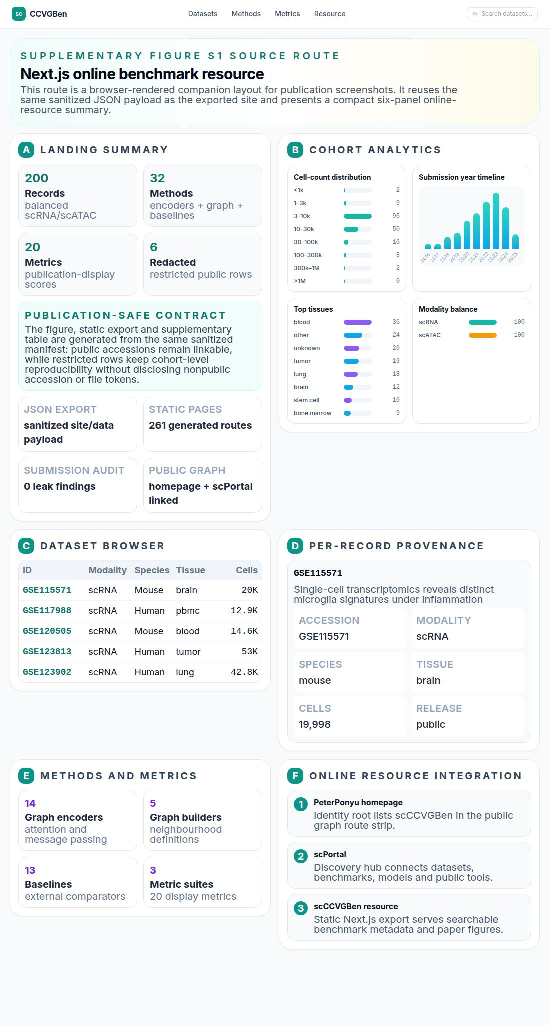
\includegraphics[width=0.78\textwidth,height=0.82\textheight,keepaspectratio]{fig_supp_nextjs.pdf}
  \caption{\textbf{Next.js interactive benchmark explorer.}
    A publication-scale rendering of the polished Next.js static-export resource.
    \textbf{(A)}~Landing summary with the benchmark counts and public-resource entry points.
    \textbf{(B)}~Cohort composition charts for modality, species and submission year.
    \textbf{(C)}~Dataset browser listing accession-safe public records with modality, species, tissue and cell-count columns.
    \textbf{(D)}~Per-record metadata view using redacted identifiers for restricted-access rows.
    \textbf{(E)}~Method and metric taxonomy cards for the 32 benchmark methods and 20 publication-display metrics.
    \textbf{(F)}~Online-resource integration panel showing how the scCCVGBen resource is linked from PeterPonyu's homepage and scPortal public graph.
    The figure is composed by the project figure script from the same sanitized JSON data that drives the static export, avoiding manual LaTeX subpanel placement.}%
  \label{figS1_nextjs}
\end{figure*}

\begin{figure*}[!htbp]
  \centering
  
\includegraphics[width=0.78\textwidth,height=0.82\textheight,keepaspectratio]{fig_online_resource_integration.pdf}
  \caption{\textbf{Online resource integration.} The deployed companion site at \url{https://peterponyu.github.io/scccvgben-next/} surfaces per-dataset metadata cards, an interactive figure browser and a public-graph integration. The benchmark cohort is registered against the broader scPortal public graph so that the dataset records reported here can be discovered alongside related single-cell tooling without cloning the source repository.
    The visual content is sourced from the route shown on the companion public page and is intended to remain legible when rendered inside the 17~cm~${\times}$~21~cm manuscript envelope.}%
  \label{figS2_online_resource}
\end{figure*}

\subsection*{Effect-size tables behind the figures (all twenty metrics)}\label{app:effects}

The tables below list the paired Wilcoxon signed-rank effect estimates and Holm-corrected $p$-values that are summarised graphically in the corresponding main-paper figures, reported across all twenty evaluation metrics (clustering compactness; UMAP and t-SNE neighbourhood preservation; intrinsic latent geometry). Effect sizes are reported as the per-dataset mean difference (reference method minus comparator); for the Davies--Bouldin index the sign convention is preserved (lower is better), so a negative value indicates the reference is better. Significance levels: $*$ $p<0.05$, $**$ $p<0.01$, $***$ $p<0.001$, ns otherwise.

% Auto-generated by scripts/compute_paper_effects.py — do not edit by hand.
% Contains fully-rendered longtables for the effect-size appendix.
% Requires: booktabs, longtable, array (loaded in main document).

% ---- fig03 part 1/1 ----
\begingroup
\scriptsize
\setlength{\tabcolsep}{2pt}
\begin{longtable}{lccc}
\caption{Effect sizes behind Fig.~\ref{fig03} (component ablation against the stochastic VAE baseline; $n=100$ paired scRNA-seq datasets per comparison). Mean difference = reference $-$ comparator; DAV: lower is better so negative = reference better.}\label{table_fig03}\\
\toprule
\textbf{Metric} & \textbf{CenVAE -- VAE} & \textbf{CouVAE -- VAE} & \textbf{GAT-VAE -- VAE} \\
\midrule
\endfirsthead
\multicolumn{4}{l}{\scriptsize\itshape (continued from previous page)} \\
\toprule
\textbf{Metric} & \textbf{CenVAE -- VAE} & \textbf{CouVAE -- VAE} & \textbf{GAT-VAE -- VAE} \\
\midrule
\endhead
\midrule
\multicolumn{4}{r}{\scriptsize\itshape (continued on next page)} \\
\endfoot
\bottomrule
\endlastfoot
\multicolumn{4}{l}{\textit{Clustering compactness (BEN)}} \\
\quad ASW $\uparrow$ & $+0.112^{***}$ & $+0.060^{***}$ & $+0.060^{***}$ \\
\quad DAV $\downarrow$ & $-0.424^{***}$ & $-0.289^{***}$ & $-0.173^{***}$ \\
\quad CAL $\uparrow$ & $+554.246^{***}$ & $+594.810^{***}$ & $+183.301^{***}$ \\
\midrule
\multicolumn{4}{l}{\textit{DRE — UMAP}} \\
\quad DC UMAP $\uparrow$ & $+0.010$\,ns & $+0.132^{***}$ & $+0.014$\,ns \\
\quad $Q_L$ UMAP $\uparrow$ & $+0.090^{***}$ & $+0.079^{***}$ & $+0.050^{***}$ \\
\quad $Q_G$ UMAP $\uparrow$ & $+0.013^{**}$ & $+0.062^{***}$ & $+0.004$\,ns \\
\quad $K_{\max}$ UMAP & $-112.822^{***}$ & $+10.978^{*}$ & $-7.689^{**}$ \\
\quad Overall UMAP $\uparrow$ & $+0.038^{***}$ & $+0.091^{***}$ & $+0.023^{***}$ \\
\midrule
\multicolumn{4}{l}{\textit{DRE — t-SNE}} \\
\quad DC t-SNE $\uparrow$ & $+0.020$\,ns & $+0.128^{***}$ & $-0.001$\,ns \\
\quad $Q_L$ t-SNE $\uparrow$ & $+0.100^{***}$ & $+0.076^{***}$ & $+0.051^{***}$ \\
\quad $Q_G$ t-SNE $\uparrow$ & $+0.017^{***}$ & $+0.063^{***}$ & $+0.005$\,ns \\
\quad $K_{\max}$ t-SNE & $-102.689^{***}$ & $+46.467^{**}$ & $+1.222$\,ns \\
\quad Overall t-SNE $\uparrow$ & $+0.046^{***}$ & $+0.089^{***}$ & $+0.018^{***}$ \\
\midrule
\multicolumn{4}{l}{\textit{LSE — intrinsic geometry}} \\
\quad Manifold dim.\ $\uparrow$ & $+0.103^{***}$ & $+0.177^{***}$ & $-0.015^{*}$ \\
\quad Spectral decay $\uparrow$ & $+0.057^{***}$ & $+0.068^{***}$ & $-0.003$\,ns \\
\quad Part.\ ratio $\uparrow$ & $+0.129^{***}$ & $+0.228^{***}$ & $-0.022^{*}$ \\
\quad Anisotropy $\uparrow$ & $+0.151^{***}$ & $+0.128^{***}$ & $-0.017^{***}$ \\
\quad Trajectory dir.\ $\uparrow$ & $+0.043^{***}$ & $+0.115^{***}$ & $+0.006$\,ns \\
\quad Noise resil.\ $\uparrow$ & $+0.035^{***}$ & $+0.108^{***}$ & $-0.001$\,ns \\
\quad Intrinsic overall $\uparrow$ & $+0.075^{***}$ & $+0.131^{***}$ & $-0.005$\,ns \\
\end{longtable}
\endgroup

% ---- fig04 part 1/1 ----
\begingroup
\scriptsize
\setlength{\tabcolsep}{2pt}
\begin{longtable}{lcccc}
\caption{Effect sizes behind Fig.~\ref{fig04} (CCVGAE joint configuration vs.\ single-component variants; reference is scCCVGBen; $n=100$ paired scRNA-seq datasets per comparison).}\label{table_fig04}\\
\toprule
\textbf{Metric} & \textbf{vs VAE} & \textbf{vs CenVAE} & \textbf{vs CouVAE} & \textbf{vs GAT-VAE} \\
\midrule
\endfirsthead
\multicolumn{5}{l}{\scriptsize\itshape (continued from previous page)} \\
\toprule
\textbf{Metric} & \textbf{vs VAE} & \textbf{vs CenVAE} & \textbf{vs CouVAE} & \textbf{vs GAT-VAE} \\
\midrule
\endhead
\midrule
\multicolumn{5}{r}{\scriptsize\itshape (continued on next page)} \\
\endfoot
\bottomrule
\endlastfoot
\multicolumn{5}{l}{\textit{Clustering compactness (BEN)}} \\
\quad ASW $\uparrow$ & $+0.288^{***}$ & $+0.177^{***}$ & $+0.231^{***}$ & $+0.224^{***}$ \\
\quad DAV $\downarrow$ & $-0.800^{***}$ & $-0.381^{***}$ & $-0.535^{***}$ & $-0.597^{***}$ \\
\quad CAL $\uparrow$ & $+4270.926^{***}$ & $+3725.693^{***}$ & $+3677.957^{***}$ & $+4076.769^{***}$ \\
\midrule
\multicolumn{5}{l}{\textit{DRE — UMAP}} \\
\quad DC UMAP $\uparrow$ & $+0.030$\,ns & $+0.020$\,ns & $-0.100^{***}$ & $+0.014$\,ns \\
\quad $Q_L$ UMAP $\uparrow$ & $+0.182^{***}$ & $+0.090^{***}$ & $+0.101^{***}$ & $+0.135^{***}$ \\
\quad $Q_G$ UMAP $\uparrow$ & $+0.022^{**}$ & $+0.008$\,ns & $-0.040^{***}$ & $+0.018^{**}$ \\
\quad $K_{\max}$ UMAP & $-236.837^{***}$ & $-130.956^{***}$ & $-258.556^{***}$ & $-211.467^{***}$ \\
\quad Overall UMAP $\uparrow$ & $+0.078^{***}$ & $+0.039^{***}$ & $-0.013$\,ns & $+0.056^{***}$ \\
\midrule
\multicolumn{5}{l}{\textit{DRE — t-SNE}} \\
\quad DC t-SNE $\uparrow$ & $+0.037$\,ns & $+0.018$\,ns & $-0.090^{***}$ & $+0.034$\,ns \\
\quad $Q_L$ t-SNE $\uparrow$ & $+0.205^{***}$ & $+0.104^{***}$ & $+0.128^{***}$ & $+0.156^{***}$ \\
\quad $Q_G$ t-SNE $\uparrow$ & $+0.032^{***}$ & $+0.014^{*}$ & $-0.031^{***}$ & $+0.028^{***}$ \\
\quad $K_{\max}$ t-SNE & $-219.985^{***}$ & $-129.111^{***}$ & $-274.022^{***}$ & $-201.822^{***}$ \\
\quad Overall t-SNE $\uparrow$ & $+0.091^{***}$ & $+0.046^{***}$ & $+0.002$\,ns & $+0.072^{***}$ \\
\midrule
\multicolumn{5}{l}{\textit{LSE — intrinsic geometry}} \\
\quad Manifold dim.\ $\uparrow$ & $+0.255^{***}$ & $+0.151^{***}$ & $+0.074^{***}$ & $+0.274^{***}$ \\
\quad Spectral decay $\uparrow$ & $+0.139^{***}$ & $+0.083^{***}$ & $+0.072^{***}$ & $+0.140^{***}$ \\
\quad Part.\ ratio $\uparrow$ & $+0.310^{***}$ & $+0.185^{***}$ & $+0.081^{***}$ & $+0.328^{***}$ \\
\quad Anisotropy $\uparrow$ & $+0.234^{***}$ & $+0.086^{***}$ & $+0.106^{***}$ & $+0.246^{***}$ \\
\quad Trajectory dir.\ $\uparrow$ & $+0.206^{***}$ & $+0.164^{***}$ & $+0.091^{***}$ & $+0.198^{***}$ \\
\quad Noise resil.\ $\uparrow$ & $+0.272^{***}$ & $+0.237^{***}$ & $+0.164^{***}$ & $+0.272^{***}$ \\
\quad Intrinsic overall $\uparrow$ & $+0.233^{***}$ & $+0.160^{***}$ & $+0.102^{***}$ & $+0.237^{***}$ \\
\end{longtable}
\endgroup

% ---- fig05 part 1/3 ----
\begingroup
\scriptsize
\setlength{\tabcolsep}{2pt}
\begin{longtable}{lcccccc}
\caption{Effect sizes behind Fig.~\ref{fig05} (encoder backbone robustness; reference is GAT, $n=100$ paired scRNA-seq datasets per comparison; positive = GAT better). Part 1 of 3.}\label{table_fig05}\\
\toprule
\textbf{Metric} & \textbf{GATv2} & \textbf{Transformer} & \textbf{SuperGAT} & \textbf{GCN} & \textbf{SAGE} & \textbf{GraphConv} \\
\midrule
\endfirsthead
\multicolumn{7}{l}{\scriptsize\itshape (continued from previous page)} \\
\toprule
\textbf{Metric} & \textbf{GATv2} & \textbf{Transformer} & \textbf{SuperGAT} & \textbf{GCN} & \textbf{SAGE} & \textbf{GraphConv} \\
\midrule
\endhead
\midrule
\multicolumn{7}{r}{\scriptsize\itshape (continued on next page)} \\
\endfoot
\bottomrule
\endlastfoot
\multicolumn{7}{l}{\textit{Clustering compactness (BEN)}} \\
\quad ASW $\uparrow$ & $-0.001$\,ns & $+0.077^{***}$ & $-0.007$\,ns & $+0.066^{***}$ & $+0.078^{***}$ & $+0.224^{***}$ \\
\quad DAV $\downarrow$ & $-0.009$\,ns & $-0.138^{***}$ & $+0.001$\,ns & $-0.127^{***}$ & $-0.142^{***}$ & $-0.381^{***}$ \\
\quad CAL $\uparrow$ & $-125.020$\,ns & $+1507.915^{***}$ & $-130.025$\,ns & $+1388.231^{***}$ & $+1594.431^{***}$ & $+4130.369^{***}$ \\
\midrule
\multicolumn{7}{l}{\textit{DRE — UMAP}} \\
\quad DC UMAP $\uparrow$ & $-0.001$\,ns & $-0.061^{***}$ & $-0.001$\,ns & $-0.030^{***}$ & $-0.067^{***}$ & $+0.074^{***}$ \\
\quad $Q_L$ UMAP $\uparrow$ & $-0.006$\,ns & $+0.020^{***}$ & $-0.003$\,ns & $+0.019^{***}$ & $+0.017^{**}$ & $+0.089^{***}$ \\
\quad $Q_G$ UMAP $\uparrow$ & $-0.003$\,ns & $-0.031^{***}$ & $-0.002$\,ns & $-0.014^{***}$ & $-0.035^{***}$ & $+0.037^{***}$ \\
\quad $K_{\max}$ UMAP & $-6.020$\,ns & $-107.280^{***}$ & $-1.940$\,ns & $-74.990^{***}$ & $-109.950^{***}$ & $+4.220$\,ns \\
\quad Overall UMAP $\uparrow$ & $-0.004$\,ns & $-0.024^{***}$ & $-0.002$\,ns & $-0.008$\,ns & $-0.028^{***}$ & $+0.067^{***}$ \\
\midrule
\multicolumn{7}{l}{\textit{DRE — t-SNE}} \\
\quad DC t-SNE $\uparrow$ & $-0.005$\,ns & $-0.049^{***}$ & $-0.018$\,ns & $-0.045^{***}$ & $-0.070^{***}$ & $+0.062^{***}$ \\
\quad $Q_L$ t-SNE $\uparrow$ & $-0.002$\,ns & $+0.036^{***}$ & $-0.001$\,ns & $+0.025^{***}$ & $+0.031^{***}$ & $+0.092^{***}$ \\
\quad $Q_G$ t-SNE $\uparrow$ & $-0.004$\,ns & $-0.022^{***}$ & $-0.006$\,ns & $-0.016^{***}$ & $-0.031^{***}$ & $+0.037^{***}$ \\
\quad $K_{\max}$ t-SNE & $-0.470$\,ns & $-129.450^{***}$ & $+3.070$\,ns & $-91.210^{***}$ & $-135.700^{***}$ & $+48.370^{***}$ \\
\quad Overall t-SNE $\uparrow$ & $-0.003$\,ns & $-0.012^{*}$ & $-0.008$\,ns & $-0.012$\,ns & $-0.024^{***}$ & $+0.064^{***}$ \\
\midrule
\multicolumn{7}{l}{\textit{LSE — intrinsic geometry}} \\
\quad Manifold dim.\ $\uparrow$ & $-0.000$\,ns & $-0.006$\,ns & $-0.000$\,ns & $+0.000$\,ns & $-0.011$\,ns & $+0.078^{***}$ \\
\quad Spectral decay $\uparrow$ & $-0.001$\,ns & $+0.001$\,ns & $-0.001$\,ns & $+0.006$\,ns & $-0.000$\,ns & $+0.034^{***}$ \\
\quad Part.\ ratio $\uparrow$ & $+0.001$\,ns & $-0.005$\,ns & $-0.001$\,ns & $+0.006$\,ns & $-0.009$\,ns & $+0.046^{***}$ \\
\quad Anisotropy $\uparrow$ & $-0.004$\,ns & $-0.004$\,ns & $-0.000$\,ns & $+0.013^{**}$ & $-0.001$\,ns & $+0.102^{***}$ \\
\quad Trajectory dir.\ $\uparrow$ & $+0.002$\,ns & $-0.006$\,ns & $+0.003$\,ns & $+0.007$\,ns & $-0.008$\,ns & $-0.006$\,ns \\
\quad Noise resil.\ $\uparrow$ & $+0.007$\,ns & $-0.031$\,ns & $-0.011$\,ns & $+0.013$\,ns & $-0.038$\,ns & $+0.154^{***}$ \\
\quad Intrinsic overall $\uparrow$ & $+0.002$\,ns & $-0.010$\,ns & $-0.002$\,ns & $+0.008$\,ns & $-0.013$\,ns & $+0.062^{***}$ \\
\end{longtable}
\endgroup

% ---- fig05 part 2/3 ----
\begingroup
\scriptsize
\setlength{\tabcolsep}{2pt}
\begin{longtable}{lcccccc}
\caption{Effect sizes behind Fig.~\ref{fig05} (encoder backbone robustness; reference is GAT, $n=100$ paired scRNA-seq datasets per comparison; positive = GAT better). Part 2 of 3.}\label{table_fig05_part2}\\
\toprule
\textbf{Metric} & \textbf{Cheb} & \textbf{TAG} & \textbf{ARMA} & \textbf{SG} & \textbf{SSG} & \textbf{GIN} \\
\midrule
\endfirsthead
\multicolumn{7}{l}{\scriptsize\itshape (continued from previous page)} \\
\toprule
\textbf{Metric} & \textbf{Cheb} & \textbf{TAG} & \textbf{ARMA} & \textbf{SG} & \textbf{SSG} & \textbf{GIN} \\
\midrule
\endhead
\midrule
\multicolumn{7}{r}{\scriptsize\itshape (continued on next page)} \\
\endfoot
\bottomrule
\endlastfoot
\multicolumn{7}{l}{\textit{Clustering compactness (BEN)}} \\
\quad ASW $\uparrow$ & $+0.192^{***}$ & $+0.063^{***}$ & $+0.209^{***}$ & $+0.037^{***}$ & $+0.049^{***}$ & $-0.023$\,ns \\
\quad DAV $\downarrow$ & $-0.479^{***}$ & $-0.116^{***}$ & $-0.457^{***}$ & $-0.062^{***}$ & $-0.091^{***}$ & $+0.002$\,ns \\
\quad CAL $\uparrow$ & $+3169.168^{***}$ & $+1299.587^{***}$ & $+3555.516^{***}$ & $+1002.104^{***}$ & $+1077.646^{***}$ & $-397.399$\,ns \\
\midrule
\multicolumn{7}{l}{\textit{DRE — UMAP}} \\
\quad DC UMAP $\uparrow$ & $-0.099^{***}$ & $-0.063^{***}$ & $+0.023$\,ns & $-0.041^{***}$ & $-0.060^{***}$ & $+0.168^{***}$ \\
\quad $Q_L$ UMAP $\uparrow$ & $+0.082^{***}$ & $+0.012^{*}$ & $+0.138^{***}$ & $-0.001$\,ns & $+0.000$\,ns & $+0.130^{***}$ \\
\quad $Q_G$ UMAP $\uparrow$ & $-0.044^{***}$ & $-0.034^{***}$ & $+0.005$\,ns & $-0.021^{***}$ & $-0.031^{***}$ & $+0.071^{***}$ \\
\quad $K_{\max}$ UMAP & $-258.400^{***}$ & $-104.350^{***}$ & $-157.280^{***}$ & $-58.840^{***}$ & $-76.060^{***}$ & $+42.755^{***}$ \\
\quad Overall UMAP $\uparrow$ & $-0.020^{**}$ & $-0.029^{***}$ & $+0.056^{**}$ & $-0.021^{***}$ & $-0.030^{***}$ & $+0.123^{***}$ \\
\midrule
\multicolumn{7}{l}{\textit{DRE — t-SNE}} \\
\quad DC t-SNE $\uparrow$ & $-0.091^{***}$ & $-0.055^{***}$ & $-0.017$\,ns & $-0.035^{**}$ & $-0.062^{***}$ & $+0.136^{***}$ \\
\quad $Q_L$ t-SNE $\uparrow$ & $+0.101^{***}$ & $+0.030^{***}$ & $+0.152^{***}$ & $+0.007^{*}$ & $+0.012^{**}$ & $+0.085^{***}$ \\
\quad $Q_G$ t-SNE $\uparrow$ & $-0.037^{***}$ & $-0.025^{***}$ & $+0.016$\,ns & $-0.016^{***}$ & $-0.027^{***}$ & $+0.047^{***}$ \\
\quad $K_{\max}$ t-SNE & $-287.310^{***}$ & $-122.060^{***}$ & $-28.320$\,ns & $-72.790^{***}$ & $-98.700^{***}$ & $+1.959^{**}$ \\
\quad Overall t-SNE $\uparrow$ & $-0.009$\,ns & $-0.017^{**}$ & $+0.050^{**}$ & $-0.015^{**}$ & $-0.026^{***}$ & $+0.089^{***}$ \\
\midrule
\multicolumn{7}{l}{\textit{LSE — intrinsic geometry}} \\
\quad Manifold dim.\ $\uparrow$ & $+0.047^{***}$ & $-0.019^{**}$ & $+0.115^{***}$ & $-0.000$\,ns & $-0.015^{*}$ & $-0.021$\,ns \\
\quad Spectral decay $\uparrow$ & $+0.041^{***}$ & $-0.008$\,ns & $-0.052^{***}$ & $-0.017^{***}$ & $-0.010$\,ns & $-0.275^{***}$ \\
\quad Part.\ ratio $\uparrow$ & $+0.028^{***}$ & $-0.016^{**}$ & $+0.016$\,ns & $-0.010$\,ns & $-0.013^{*}$ & $-0.007$\,ns \\
\quad Anisotropy $\uparrow$ & $+0.077^{***}$ & $-0.010$\,ns & $-0.128^{***}$ & $-0.018^{**}$ & $-0.009$\,ns & $-0.386^{***}$ \\
\quad Trajectory dir.\ $\uparrow$ & $+0.022$\,ns & $-0.024$\,ns & $-0.047^{*}$ & $-0.015$\,ns & $-0.016$\,ns & $-0.246^{***}$ \\
\quad Noise resil.\ $\uparrow$ & $+0.103^{***}$ & $-0.086^{***}$ & $+0.087$\,ns & $-0.024$\,ns & $-0.063^{*}$ & $-0.389^{***}$ \\
\quad Intrinsic overall $\uparrow$ & $+0.051^{***}$ & $-0.031^{**}$ & $-0.003$\,ns & $-0.015$\,ns & $-0.023$\,ns & $-0.238^{***}$ \\
\end{longtable}
\endgroup

% ---- fig05 part 3/3 ----
\begingroup
\scriptsize
\setlength{\tabcolsep}{2pt}
\begin{longtable}{lc}
\caption{Effect sizes behind Fig.~\ref{fig05} (encoder backbone robustness; reference is GAT, $n=100$ paired scRNA-seq datasets per comparison; positive = GAT better). Part 3 of 3.}\label{table_fig05_part3}\\
\toprule
\textbf{Metric} & \textbf{EdgeConv} \\
\midrule
\endfirsthead
\multicolumn{2}{l}{\scriptsize\itshape (continued from previous page)} \\
\toprule
\textbf{Metric} & \textbf{EdgeConv} \\
\midrule
\endhead
\midrule
\multicolumn{2}{r}{\scriptsize\itshape (continued on next page)} \\
\endfoot
\bottomrule
\endlastfoot
\multicolumn{2}{l}{\textit{Clustering compactness (BEN)}} \\
\quad ASW $\uparrow$ & $+0.139^{***}$ \\
\quad DAV $\downarrow$ & $-0.294^{***}$ \\
\quad CAL $\uparrow$ & $-360.755$\,ns \\
\midrule
\multicolumn{2}{l}{\textit{DRE — UMAP}} \\
\quad DC UMAP $\uparrow$ & $-0.115^{***}$ \\
\quad $Q_L$ UMAP $\uparrow$ & $+0.040^{***}$ \\
\quad $Q_G$ UMAP $\uparrow$ & $-0.052^{***}$ \\
\quad $K_{\max}$ UMAP & $-169.330^{***}$ \\
\quad Overall UMAP $\uparrow$ & $-0.043^{***}$ \\
\midrule
\multicolumn{2}{l}{\textit{DRE — t-SNE}} \\
\quad DC t-SNE $\uparrow$ & $-0.091^{***}$ \\
\quad $Q_L$ t-SNE $\uparrow$ & $+0.054^{***}$ \\
\quad $Q_G$ t-SNE $\uparrow$ & $-0.033^{***}$ \\
\quad $K_{\max}$ t-SNE & $-170.480^{***}$ \\
\quad Overall t-SNE $\uparrow$ & $-0.023^{***}$ \\
\midrule
\multicolumn{2}{l}{\textit{LSE — intrinsic geometry}} \\
\quad Manifold dim.\ $\uparrow$ & $+0.003$\,ns \\
\quad Spectral decay $\uparrow$ & $-0.154^{***}$ \\
\quad Part.\ ratio $\uparrow$ & $-0.087^{***}$ \\
\quad Anisotropy $\uparrow$ & $-0.267^{***}$ \\
\quad Trajectory dir.\ $\uparrow$ & $-0.183^{***}$ \\
\quad Noise resil.\ $\uparrow$ & $-0.399^{***}$ \\
\quad Intrinsic overall $\uparrow$ & $-0.198^{***}$ \\
\end{longtable}
\endgroup

% ---- fig06 part 1/1 ----
\begingroup
\scriptsize
\setlength{\tabcolsep}{2pt}
\begin{longtable}{lcccc}
\caption{Effect sizes behind Fig.~\ref{fig06} (graph-construction robustness; reference is kNN-Euclidean, $n=100$ paired scRNA-seq datasets per comparison).}\label{table_fig06}\\
\toprule
\textbf{Metric} & \textbf{kNN-cosine} & \textbf{SNN} & \textbf{mutual-kNN} & \textbf{Gaussian-thresh.} \\
\midrule
\endfirsthead
\multicolumn{5}{l}{\scriptsize\itshape (continued from previous page)} \\
\toprule
\textbf{Metric} & \textbf{kNN-cosine} & \textbf{SNN} & \textbf{mutual-kNN} & \textbf{Gaussian-thresh.} \\
\midrule
\endhead
\midrule
\multicolumn{5}{r}{\scriptsize\itshape (continued on next page)} \\
\endfoot
\bottomrule
\endlastfoot
\multicolumn{5}{l}{\textit{Clustering compactness (BEN)}} \\
\quad ASW $\uparrow$ & $-0.050^{***}$ & $-0.095^{***}$ & $+0.042^{***}$ & $+0.013$\,ns \\
\quad DAV $\downarrow$ & $+0.045^{***}$ & $+0.125^{***}$ & $-0.127^{***}$ & $-0.228^{***}$ \\
\quad CAL $\uparrow$ & $-1516.711^{***}$ & $-2863.534^{***}$ & $+1409.980^{***}$ & $+1601.160^{***}$ \\
\midrule
\multicolumn{5}{l}{\textit{DRE — UMAP}} \\
\quad DC UMAP $\uparrow$ & $+0.011$\,ns & $+0.037^{**}$ & $-0.026^{*}$ & $+0.035^{*}$ \\
\quad $Q_L$ UMAP $\uparrow$ & $+0.005$\,ns & $-0.013^{**}$ & $+0.056^{***}$ & $+0.071^{***}$ \\
\quad $Q_G$ UMAP $\uparrow$ & $+0.003$\,ns & $+0.013^{***}$ & $-0.005$\,ns & $+0.013^{*}$ \\
\quad $K_{\max}$ UMAP & $-16.969$\,ns & $+27.031^{***}$ & $-82.724^{***}$ & $-94.837^{***}$ \\
\quad Overall UMAP $\uparrow$ & $+0.006$\,ns & $+0.012^{*}$ & $+0.008$\,ns & $+0.040^{***}$ \\
\midrule
\multicolumn{5}{l}{\textit{DRE — t-SNE}} \\
\quad DC t-SNE $\uparrow$ & $+0.017$\,ns & $+0.067^{***}$ & $-0.028^{*}$ & $+0.030^{*}$ \\
\quad $Q_L$ t-SNE $\uparrow$ & $-0.000$\,ns & $-0.029^{***}$ & $+0.042^{***}$ & $+0.054^{***}$ \\
\quad $Q_G$ t-SNE $\uparrow$ & $+0.006^{*}$ & $+0.020^{***}$ & $-0.008^{*}$ & $+0.014^{**}$ \\
\quad $K_{\max}$ t-SNE & $-26.408^{***}$ & $+20.694$\,ns & $-90.582^{***}$ & $-87.388^{***}$ \\
\quad Overall t-SNE $\uparrow$ & $+0.007$\,ns & $+0.019^{**}$ & $+0.002$\,ns & $+0.033^{***}$ \\
\midrule
\multicolumn{5}{l}{\textit{LSE — intrinsic geometry}} \\
\quad Manifold dim.\ $\uparrow$ & $-0.003$\,ns & $-0.002$\,ns & $+0.010$\,ns & $+0.033^{***}$ \\
\quad Spectral decay $\uparrow$ & $-0.010^{**}$ & $-0.017^{***}$ & $+0.013^{***}$ & $+0.032^{***}$ \\
\quad Part.\ ratio $\uparrow$ & $-0.007$\,ns & $-0.008$\,ns & $+0.003$\,ns & $+0.023^{***}$ \\
\quad Anisotropy $\uparrow$ & $-0.012^{**}$ & $-0.019^{***}$ & $+0.029^{***}$ & $+0.058^{***}$ \\
\quad Trajectory dir.\ $\uparrow$ & $-0.013$\,ns & $-0.017$\,ns & $-0.000$\,ns & $+0.024^{**}$ \\
\quad Noise resil.\ $\uparrow$ & $-0.040$\,ns & $-0.017$\,ns & $+0.027$\,ns & $+0.091^{***}$ \\
\quad Intrinsic overall $\uparrow$ & $-0.016$\,ns & $-0.014$\,ns & $+0.012$\,ns & $+0.044^{***}$ \\
\end{longtable}
\endgroup

% ---- fig07 part 1/2 ----
\begingroup
\scriptsize
\setlength{\tabcolsep}{2pt}
\begin{longtable}{lcccccc}
\caption{Effect sizes behind Fig.~\ref{fig07} (cross-method benchmark on scRNA-seq; reference is scCCVGBen; paired-$n$ varies by comparator and is shown in parentheses). Part 1 of 2.}\label{table_fig07}\\
\toprule
\textbf{Metric} & \textbf{PCA (94)} & \textbf{KPCA (94)} & \textbf{ICA (46)} & \textbf{FA (92)} & \textbf{NMF (94)} & \textbf{TSVD (94)} \\
\midrule
\endfirsthead
\multicolumn{7}{l}{\scriptsize\itshape (continued from previous page)} \\
\toprule
\textbf{Metric} & \textbf{PCA (94)} & \textbf{KPCA (94)} & \textbf{ICA (46)} & \textbf{FA (92)} & \textbf{NMF (94)} & \textbf{TSVD (94)} \\
\midrule
\endhead
\midrule
\multicolumn{7}{r}{\scriptsize\itshape (continued on next page)} \\
\endfoot
\bottomrule
\endlastfoot
\multicolumn{7}{l}{\textit{Clustering compactness (BEN)}} \\
\quad ASW $\uparrow$ & $+0.162^{***}$ & $+0.164^{***}$ & $+0.208^{***}$ & $+0.070^{***}$ & $+0.114^{***}$ & $+0.164^{***}$ \\
\quad DAV $\downarrow$ & $-0.433^{***}$ & $-0.432^{***}$ & $-0.485^{***}$ & $-0.035$\,ns & $-0.257^{***}$ & $-0.432^{***}$ \\
\quad CAL $\uparrow$ & $+3895.767^{***}$ & $+3903.251^{***}$ & $+4497.773^{***}$ & $+4312.013^{***}$ & $+3904.654^{***}$ & $+3864.598^{***}$ \\
\midrule
\multicolumn{7}{l}{\textit{DRE — UMAP}} \\
\quad DC UMAP $\uparrow$ & $+0.052^{**}$ & $+0.054^{**}$ & $+0.260^{***}$ & $+0.191^{***}$ & $+0.140^{***}$ & $+0.051^{**}$ \\
\quad $Q_L$ UMAP $\uparrow$ & $+0.113^{***}$ & $+0.111^{***}$ & $+0.149^{***}$ & $+0.098^{***}$ & $+0.097^{***}$ & $+0.114^{***}$ \\
\quad $Q_G$ UMAP $\uparrow$ & $+0.026^{***}$ & $+0.027^{***}$ & $+0.093^{***}$ & $+0.063^{***}$ & $+0.055^{***}$ & $+0.025^{***}$ \\
\quad $K_{\max}$ UMAP & $-120.670^{***}$ & $-115.926^{***}$ & $-71.957^{***}$ & $-67.713^{***}$ & $-68.362^{***}$ & $-122.670^{***}$ \\
\quad Overall UMAP $\uparrow$ & $+0.064^{***}$ & $+0.064^{***}$ & $+0.167^{***}$ & $+0.117^{***}$ & $+0.097^{***}$ & $+0.063^{***}$ \\
\midrule
\multicolumn{7}{l}{\textit{DRE — t-SNE}} \\
\quad DC t-SNE $\uparrow$ & $+0.039^{*}$ & $+0.040^{*}$ & $+0.239^{***}$ & $+0.187^{***}$ & $+0.122^{***}$ & $+0.040^{*}$ \\
\quad $Q_L$ t-SNE $\uparrow$ & $+0.117^{***}$ & $+0.114^{***}$ & $+0.151^{***}$ & $+0.098^{***}$ & $+0.095^{***}$ & $+0.119^{***}$ \\
\quad $Q_G$ t-SNE $\uparrow$ & $+0.026^{***}$ & $+0.025^{***}$ & $+0.095^{***}$ & $+0.062^{***}$ & $+0.052^{***}$ & $+0.026^{***}$ \\
\quad $K_{\max}$ t-SNE & $-117.372^{***}$ & $-117.074^{***}$ & $-59.304^{***}$ & $-70.074^{***}$ & $-59.755^{***}$ & $-116.989^{***}$ \\
\quad Overall t-SNE $\uparrow$ & $+0.061^{***}$ & $+0.060^{***}$ & $+0.162^{***}$ & $+0.116^{***}$ & $+0.090^{***}$ & $+0.062^{***}$ \\
\midrule
\multicolumn{7}{l}{\textit{LSE — intrinsic geometry}} \\
\quad Manifold dim.\ $\uparrow$ & $+0.195^{***}$ & $+0.197^{***}$ & $+0.390^{***}$ & $+0.463^{***}$ & $+0.343^{***}$ & $+0.198^{***}$ \\
\quad Spectral decay $\uparrow$ & $+0.108^{***}$ & $+0.109^{***}$ & $+0.241^{***}$ & $+0.255^{***}$ & $+0.148^{***}$ & $+0.105^{***}$ \\
\quad Part.\ ratio $\uparrow$ & $+0.212^{***}$ & $+0.214^{***}$ & $+0.672^{***}$ & $+0.708^{***}$ & $+0.376^{***}$ & $+0.205^{***}$ \\
\quad Anisotropy $\uparrow$ & $+0.229^{***}$ & $+0.231^{***}$ & $+0.471^{***}$ & $+0.490^{***}$ & $+0.195^{***}$ & $+0.214^{***}$ \\
\quad Trajectory dir.\ $\uparrow$ & $+0.109^{***}$ & $+0.110^{***}$ & $+0.337^{***}$ & $+0.375^{***}$ & $+0.221^{***}$ & $+0.106^{***}$ \\
\quad Noise resil.\ $\uparrow$ & $+0.286^{***}$ & $+0.286^{***}$ & $+0.306^{***}$ & $+0.406^{***}$ & $+0.345^{***}$ & $+0.283^{***}$ \\
\quad Intrinsic overall $\uparrow$ & $+0.183^{***}$ & $+0.184^{***}$ & $+0.384^{***}$ & $+0.433^{***}$ & $+0.268^{***}$ & $+0.179^{***}$ \\
\end{longtable}
\endgroup

% ---- fig07 part 2/2 ----
\begingroup
\scriptsize
\setlength{\tabcolsep}{2pt}
\begin{longtable}{lcccccc}
\caption{Effect sizes behind Fig.~\ref{fig07} (cross-method benchmark on scRNA-seq; reference is scCCVGBen; paired-$n$ varies by comparator and is shown in parentheses). Part 2 of 2.}\label{table_fig07_part2}\\
\toprule
\textbf{Metric} & \textbf{DICL (94)} & \textbf{scVI (48)} & \textbf{DIP (48)} & \textbf{INFO (48)} & \textbf{TC (48)} & \textbf{highBeta (48)} \\
\midrule
\endfirsthead
\multicolumn{7}{l}{\scriptsize\itshape (continued from previous page)} \\
\toprule
\textbf{Metric} & \textbf{DICL (94)} & \textbf{scVI (48)} & \textbf{DIP (48)} & \textbf{INFO (48)} & \textbf{TC (48)} & \textbf{highBeta (48)} \\
\midrule
\endhead
\midrule
\multicolumn{7}{r}{\scriptsize\itshape (continued on next page)} \\
\endfoot
\bottomrule
\endlastfoot
\multicolumn{7}{l}{\textit{Clustering compactness (BEN)}} \\
\quad ASW $\uparrow$ & $+0.024^{***}$ & $+0.341^{***}$ & $+0.266^{***}$ & $+0.224^{***}$ & $+0.226^{***}$ & $+0.175^{***}$ \\
\quad DAV $\downarrow$ & $-0.109^{***}$ & $-1.089^{***}$ & $-0.670^{***}$ & $-0.547^{***}$ & $-0.556^{***}$ & $-0.404^{***}$ \\
\quad CAL $\uparrow$ & $+3711.521^{***}$ & $+4626.168^{***}$ & $+4324.325^{***}$ & $+4016.917^{***}$ & $+3955.179^{***}$ & $+3364.267^{***}$ \\
\midrule
\multicolumn{7}{l}{\textit{DRE — UMAP}} \\
\quad DC UMAP $\uparrow$ & $+0.136^{***}$ & $+0.283^{***}$ & $+0.228^{***}$ & $+0.130^{***}$ & $+0.082^{***}$ & $+0.049^{**}$ \\
\quad $Q_L$ UMAP $\uparrow$ & $+0.060^{***}$ & $+0.249^{***}$ & $+0.189^{***}$ & $+0.142^{***}$ & $+0.144^{***}$ & $+0.106^{***}$ \\
\quad $Q_G$ UMAP $\uparrow$ & $+0.057^{***}$ & $+0.105^{***}$ & $+0.090^{***}$ & $+0.046^{***}$ & $+0.034^{***}$ & $+0.014$\,ns \\
\quad $K_{\max}$ UMAP & $-20.936^{**}$ & $-103.979^{***}$ & $-80.875^{***}$ & $-111.271^{***}$ & $-121.479^{***}$ & $-123.750^{***}$ \\
\quad Overall UMAP $\uparrow$ & $+0.085^{***}$ & $+0.212^{***}$ & $+0.169^{***}$ & $+0.106^{***}$ & $+0.087^{***}$ & $+0.056^{***}$ \\
\midrule
\multicolumn{7}{l}{\textit{DRE — t-SNE}} \\
\quad DC t-SNE $\uparrow$ & $+0.128^{***}$ & $+0.265^{***}$ & $+0.235^{***}$ & $+0.104^{***}$ & $+0.078^{***}$ & $+0.035$\,ns \\
\quad $Q_L$ t-SNE $\uparrow$ & $+0.046^{***}$ & $+0.259^{***}$ & $+0.191^{***}$ & $+0.157^{***}$ & $+0.157^{***}$ & $+0.122^{***}$ \\
\quad $Q_G$ t-SNE $\uparrow$ & $+0.056^{***}$ & $+0.112^{***}$ & $+0.098^{***}$ & $+0.047^{***}$ & $+0.041^{***}$ & $+0.019^{*}$ \\
\quad $K_{\max}$ t-SNE & $-1.606$\,ns & $-42.396^{***}$ & $-52.500^{***}$ & $-76.312^{***}$ & $-87.292^{***}$ & $-115.938^{***}$ \\
\quad Overall t-SNE $\uparrow$ & $+0.077^{***}$ & $+0.212^{***}$ & $+0.175^{***}$ & $+0.103^{***}$ & $+0.092^{***}$ & $+0.059^{***}$ \\
\midrule
\multicolumn{7}{l}{\textit{LSE — intrinsic geometry}} \\
\quad Manifold dim.\ $\uparrow$ & $+0.356^{***}$ & $+0.314^{***}$ & $+0.433^{***}$ & $+0.239^{***}$ & $+0.206^{***}$ & $+0.139^{***}$ \\
\quad Spectral decay $\uparrow$ & $+0.148^{***}$ & $+0.201^{***}$ & $+0.159^{***}$ & $+0.112^{***}$ & $+0.101^{***}$ & $+0.080^{***}$ \\
\quad Part.\ ratio $\uparrow$ & $+0.372^{***}$ & $+0.595^{***}$ & $+0.532^{***}$ & $+0.285^{***}$ & $+0.246^{***}$ & $+0.179^{***}$ \\
\quad Anisotropy $\uparrow$ & $+0.181^{***}$ & $+0.392^{***}$ & $-0.048^{***}$ & $+0.154^{***}$ & $+0.141^{***}$ & $+0.097^{***}$ \\
\quad Trajectory dir.\ $\uparrow$ & $+0.216^{***}$ & $+0.277^{***}$ & $+0.292^{***}$ & $+0.178^{***}$ & $+0.162^{***}$ & $+0.142^{***}$ \\
\quad Noise resil.\ $\uparrow$ & $+0.352^{***}$ & $+0.299^{***}$ & $+0.282^{***}$ & $+0.236^{***}$ & $+0.224^{***}$ & $+0.205^{***}$ \\
\quad Intrinsic overall $\uparrow$ & $+0.267^{***}$ & $+0.331^{***}$ & $+0.278^{***}$ & $+0.199^{***}$ & $+0.180^{***}$ & $+0.146^{***}$ \\
\end{longtable}
\endgroup

% ---- fig08 part 1/1 ----
\begingroup
\scriptsize
\setlength{\tabcolsep}{2pt}
\begin{longtable}{lccc}
\caption{Effect sizes behind Fig.~\ref{fig08} (cross-method benchmark on scATAC-seq; reference is scCCVGBen; $n=100$ paired datasets per comparison).}\label{table_fig08}\\
\toprule
\textbf{Metric} & \textbf{LSI} & \textbf{PeakVI} & \textbf{PoissonVI} \\
\midrule
\endfirsthead
\multicolumn{4}{l}{\scriptsize\itshape (continued from previous page)} \\
\toprule
\textbf{Metric} & \textbf{LSI} & \textbf{PeakVI} & \textbf{PoissonVI} \\
\midrule
\endhead
\midrule
\multicolumn{4}{r}{\scriptsize\itshape (continued on next page)} \\
\endfoot
\bottomrule
\endlastfoot
\multicolumn{4}{l}{\textit{Clustering compactness (BEN)}} \\
\quad ASW $\uparrow$ & $+0.120^{***}$ & $+0.139^{***}$ & $-0.027^{**}$ \\
\quad DAV $\downarrow$ & $-0.526^{***}$ & $-0.651^{***}$ & $+0.125^{***}$ \\
\quad CAL $\uparrow$ & $+2501.553^{***}$ & $+2663.540^{***}$ & $+689.705^{***}$ \\
\midrule
\multicolumn{4}{l}{\textit{DRE — UMAP}} \\
\quad DC UMAP $\uparrow$ & $+0.115^{***}$ & $+0.165^{***}$ & $+0.055^{***}$ \\
\quad $Q_L$ UMAP $\uparrow$ & $+0.144^{***}$ & $+0.169^{***}$ & $-0.037^{**}$ \\
\quad $Q_G$ UMAP $\uparrow$ & $+0.057^{***}$ & $+0.081^{***}$ & $+0.010^{*}$ \\
\quad $K_{\max}$ UMAP & $-103.450^{***}$ & $-111.890^{***}$ & $+66.070^{***}$ \\
\quad Overall UMAP $\uparrow$ & $+0.105^{***}$ & $+0.138^{***}$ & $+0.009$\,ns \\
\midrule
\multicolumn{4}{l}{\textit{DRE — t-SNE}} \\
\quad DC t-SNE $\uparrow$ & $+0.101^{***}$ & $+0.168^{***}$ & $+0.031^{*}$ \\
\quad $Q_L$ t-SNE $\uparrow$ & $+0.133^{***}$ & $+0.172^{***}$ & $-0.045^{***}$ \\
\quad $Q_G$ t-SNE $\uparrow$ & $+0.052^{***}$ & $+0.099^{***}$ & $+0.002$\,ns \\
\quad $K_{\max}$ t-SNE & $-117.440^{***}$ & $+32.900$\,ns & $+37.370$\,ns \\
\quad Overall t-SNE $\uparrow$ & $+0.095^{***}$ & $+0.146^{***}$ & $-0.004$\,ns \\
\midrule
\multicolumn{4}{l}{\textit{LSE — intrinsic geometry}} \\
\quad Manifold dim.\ $\uparrow$ & $+0.248^{***}$ & $+0.312^{***}$ & $+0.049^{***}$ \\
\quad Spectral decay $\uparrow$ & $+0.149^{***}$ & $+0.166^{***}$ & $+0.028^{***}$ \\
\quad Part.\ ratio $\uparrow$ & $+0.294^{***}$ & $+0.380^{***}$ & $+0.096^{***}$ \\
\quad Anisotropy $\uparrow$ & $+0.267^{***}$ & $+0.245^{***}$ & $-0.051^{**}$ \\
\quad Trajectory dir.\ $\uparrow$ & $+0.250^{***}$ & $+0.324^{***}$ & $+0.164^{***}$ \\
\quad Noise resil.\ $\uparrow$ & $+0.519^{***}$ & $+0.554^{***}$ & $+0.253^{***}$ \\
\quad Intrinsic overall $\uparrow$ & $+0.299^{***}$ & $+0.346^{***}$ & $+0.115^{***}$ \\
\end{longtable}
\endgroup



\end{appendices}

%%%%%%%%%%%%%%%%%%%%%%%%%%%%%%%%%%%%%%%%%%%%%%%%%%%%%%%%%%%%%%%%%%%%%%
%% References
%%%%%%%%%%%%%%%%%%%%%%%%%%%%%%%%%%%%%%%%%%%%%%%%%%%%%%%%%%%%%%%%%%%%%%

\begin{thebibliography}{99}

\bibitem{lopez2018deep}
Lopez R, Regier J, Cole MB, Jordan MI, Yosef N. Deep generative modeling for single-cell transcriptomics. Nat Methods. 2018;15(12):1053--1058. doi:10.1038/s41592-018-0229-2.

\bibitem{gayoso2021joint}
Gayoso A, Steier Z, Lopez R, Regier J, Nazor KL, Streets A, Yosef N. Joint probabilistic modeling of single-cell multi-omic data with totalVI. Nat Methods. 2021;18(3):272--282. doi:10.1038/s41592-020-01050-x.

\bibitem{xu2021deep}
Xu C, Lopez R, Mehlman E, Regier J, Jordan MI, Yosef N. Probabilistic harmonization and annotation of single-cell transcriptomics data with deep generative models. Mol Syst Biol. 2021;17(1):e9620. doi:10.15252/msb.20209620.

\bibitem{wang2021scgnn}
Wang J, Ma A, Chang Y, Gong J, Jiang Y, Qi R, Wang C, Fu H, Ma Q, Xu D. scGNN is a novel graph neural network framework for single-cell RNA-Seq analyses. Nat Commun. 2021;12(1):1882. doi:10.1038/s41467-021-22197-x.

\bibitem{liao2023deep}
Liao M, Liu Y, Yuan Y, Wang Y, Liu M, Wang T, Tian H, Pang L, Zhang H, Han J, Liu L. Deep graph attention autoencoder for single-cell RNA-seq clustering. Brief Bioinform. 2023;24(4):bbad174. doi:10.1093/bib/bbad174.

\bibitem{laghaee2024scvag}
Laghaee S, Mohammadi M, Razaghi-Moghadam Z, Nikoloski Z. scVAG: a unified single-cell embedder via variational graph autoencoders. Bioinformatics. 2024;40(7):btae416. doi:10.1093/bioinformatics/btae416.

\bibitem{lv2024ssgate}
Lv H, Lu J, Yu M, Sun H, Liu X. SSGATE: a self-supervised graph attention auto-encoder for single-cell multi-omics integration. Brief Bioinform. 2024;25(3):bbae188. doi:10.1093/bib/bbae188.

\bibitem{cui2024scgpt}
Cui H, Wang C, Maan H, Pang K, Luo F, Duan N, Wang B. scGPT: toward building a foundation model for single-cell multi-omics using generative AI. Nat Methods. 2024;21(8):1470--1480. doi:10.1038/s41592-024-02201-0.

\bibitem{theodoris2023geneformer}
Theodoris CV, Xiao L, Chopra A, Chaffin MD, Al Sayed ZR, Hill MC, Mantineo H, Brydon EM, Zeng Z, Liu XS, Ellinor PT. Transfer learning enables predictions in network biology. Nature. 2023;618(7965):616--624. doi:10.1038/s41586-023-06139-9.

\bibitem{lin2022scjoint}
Lin Y, Wu TY, Wan S, Yang JYH, Wong WH, Wang YXR. scJoint integrates atlas-scale single-cell RNA-seq and ATAC-seq data with transfer learning. Nat Biotechnol. 2022;40(5):703--710. doi:10.1038/s41587-021-01161-6.

\bibitem{li2024moh}
Li Y, Zheng T, Wang L, Liu X, Zhang Y. MoH: heterogeneous-graph attention network for single-cell multi-omics integration. Brief Bioinform. 2024;25(4):bbae278. doi:10.1093/bib/bbae278.

\bibitem{cao2022glue}
Cao ZJ, Gao G. Multi-omics single-cell data integration and regulatory inference with graph-linked embedding. Nat Biotechnol. 2022;40(10):1458--1466. doi:10.1038/s41587-022-01284-4.

\bibitem{luecken2022benchmarking}
Luecken MD, B\"{u}ttner M, Chaichoompu K, Danese A, Interlandi M, M\"{u}ller MF, Strobl DC, Zappia L, Dugas M, Colom\'e-Tatch\'e M, Theis FJ. Benchmarking atlas-level data integration in single-cell genomics. Nat Methods. 2022;19(1):41--50. doi:10.1038/s41592-021-01336-8.

\bibitem{stuart2019integrative}
Stuart T, Butler A, Hoffman P, Hafemeister C, Papalexi E, Mauck WM 3rd, Hao Y, Stoeckius M, Smibert P, Satija R. Comprehensive integration of single-cell data. Cell. 2019;177(7):1888--1902.e21. doi:10.1016/j.cell.2019.05.031.

\bibitem{ma2020single}
Ma Q, Xu D. Deep learning shapes single-cell data analysis. Nat Rev Mol Cell Biol. 2022;23(5):303--304. doi:10.1038/s41580-022-00466-x.

\bibitem{li2025gnnreview}
Li J, Sun Y, Yu W, Liu Y, Lu W. Graph neural networks for single-cell omics: methods, applications, and outlook. Brief Bioinform. 2025;26(1):bbae596. doi:10.1093/bib/bbae596.

\bibitem{ge2025dlreview}
Ge S, Wang H, Alavi A, Xing EP, Bar-Joseph Z. Deep learning for single-cell sequencing: a review of methods, applications, and frontiers. Genome Biol. 2025;26(1):54. doi:10.1186/s13059-025-03489-7.

\bibitem{tran2020benchmark}
Tran HTN, Ang KS, Chevrier M, Zhang X, Lee NYS, Goh M, Chen J. A benchmark of batch-effect correction methods for single-cell RNA sequencing data. Genome Biol. 2020;21(1):12. doi:10.1186/s13059-019-1850-9.

\bibitem{duo2018comparison}
Duo A, Robinson MD, Soneson C. A systematic performance evaluation of clustering methods for single-cell RNA-seq data. F1000Res. 2018;7:1141. doi:10.12688/f1000research.15666.3.

\bibitem{saelens2019comparison}
Saelens W, Cannoodt R, Todorov H, Saeys Y. A comparison of single-cell trajectory inference methods. Nat Biotechnol. 2019;37(5):547--554. doi:10.1038/s41587-019-0071-9.

\bibitem{kipf2016vgae}
Kipf TN, Welling M. Variational graph auto-encoders. NeurIPS Bayesian Deep Learning Workshop. 2016. arXiv:1611.07308. doi:10.48550/arXiv.1611.07308.

\bibitem{kingma2014vae}
Kingma DP, Welling M. Auto-encoding variational Bayes. International Conference on Learning Representations (ICLR). 2014. arXiv:1312.6114. doi:10.48550/arXiv.1312.6114.

\bibitem{velickovic2018gat}
Veli\v{c}kovi\'c P, Cucurull G, Casanova A, Romero A, Li\`o P, Bengio Y. Graph attention networks. International Conference on Learning Representations (ICLR). 2018. arXiv:1710.10903. doi:10.48550/arXiv.1710.10903.

\bibitem{higgins2017betavae}
Higgins I, Matthey L, Pal A, Burgess CP, Glorot X, Botvinick M, Mohamed S, Lerchner A. beta-VAE: learning basic visual concepts with a constrained variational framework. International Conference on Learning Representations (ICLR). 2017.

\bibitem{chen2018isolating}
Chen RTQ, Li X, Grosse RB, Duvenaud DK. Isolating sources of disentanglement in variational autoencoders. Advances in Neural Information Processing Systems (NeurIPS). 2018;31.

\bibitem{kim2018disentangling}
Kim H, Mnih A. Disentangling by factorising. International Conference on Machine Learning (ICML). 2018.

\bibitem{halko2011finding}
Halko N, Martinsson PG, Tropp JA. Finding structure with randomness: probabilistic algorithms for constructing approximate matrix decompositions. SIAM Rev. 2011;53(2):217--288. doi:10.1137/090771806.

\bibitem{wang2018dicl}
Wang Z, Wang T. Deep information clustering by latent subspace disentanglement. Proceedings of the AAAI Conference on Artificial Intelligence. 2018;32(1).

\bibitem{kumar2018dipvae}
Kumar A, Sattigeri P, Balakrishnan A. Variational inference of disentangled latent concepts from unlabeled observations. International Conference on Learning Representations (ICLR). 2018.

\bibitem{zhao2019infovae}
Zhao S, Song J, Ermon S. InfoVAE: balancing learning and inference in variational autoencoders. Proceedings of the AAAI Conference on Artificial Intelligence. 2019;33(1):5885--5892.

\bibitem{stuart2021atac}
Stuart T, Srivastava A, Madad S, Lareau CA, Satija R. Single-cell chromatin state analysis with Signac. Nat Methods. 2021;18(11):1333--1341. doi:10.1038/s41592-021-01282-5.

\bibitem{ashuach2022peakvi}
Ashuach T, Reidenbach DA, Gayoso A, Yosef N. PeakVI: a deep generative model for single-cell chromatin accessibility analysis. Cell Rep Methods. 2022;2(3):100182. doi:10.1016/j.crmeth.2022.100182.

\bibitem{martens2024poissonvi}
Martens LD, Fischer DS, Yepez VA, Theis FJ, Gagneur J. Modeling fragment counts improves single-cell ATAC-seq analysis. Nat Methods. 2024;21(1):28--31. doi:10.1038/s41592-023-02112-6.

\bibitem{mcalpine2019sleep}
McAlpine CS, Kiss MG, Rattik S, He S, Vassalli A, Valet C, Anzai A, Chan CT, Mindur JE, Kahles F, Poller WC, Frodermann V, Fenn AM, Gregory AF, Halle L, Iwamoto Y, Hoyer FF, Binder CJ, Libby P, Tafti M, Scammell TE, Nahrendorf M, Swirski FK. Sleep modulates haematopoiesis and protects against atherosclerosis. Nature. 2019;566(7744):383--387. doi:10.1038/s41586-019-0948-2.

\bibitem{wang2024sleep}
Wang Z, Liu Y, Sun M, Wang J. Sleep deprivation reshapes bone marrow hematopoiesis: a single-cell atlas. iScience. 2024;27(8):110321. doi:10.1016/j.isci.2024.110321.

\bibitem{kaushansky1994thrombopoietin}
Kaushansky K, Lok S, Holly RD, Broudy VC, Lin NL, Bailey MC, Forstrom JW, Buddle MM, Oort PJ, Hagen FS, Roth GJ, Papayannopoulou T, Foster DC. Promotion of megakaryocyte progenitor expansion and differentiation by the c-Mpl ligand thrombopoietin. Nature. 1994;369(6481):568--571. doi:10.1038/369568a0.

\bibitem{de_sauvage1994stimulation}
de Sauvage FJ, Hass PE, Spencer SD, Malloy BE, Gurney AL, Spencer SA, Darbonne WC, Henzel WJ, Wong SC, Kuang WJ, Oles KJ, Hultgren B, Solberg LA Jr, Goeddel DV, Eaton DL. Stimulation of megakaryocytopoiesis and thrombopoiesis by the c-Mpl ligand. Nature. 1994;369(6481):533--538. doi:10.1038/369533a0.

\bibitem{lok1994cloning}
Lok S, Kaushansky K, Holly RD, Kuijper JL, Lofton-Day CE, Oort PJ, Grant FJ, Heipel MD, Burkhead SK, Kramer JM, Bell LA, Sprecher CA, Blumberg H, Johnson R, Prunkard D, Ching AFT, Mathewes SL, Bailey MC, Forstrom JW, Buddle MM, Osborn SG, Evans SJ, Sheppard PO, Presnell SR, O'Hara PJ, Hagen FS, Roth GJ, Foster DC. Cloning and expression of murine thrombopoietin cDNA and stimulation of platelet production in vivo. Nature. 1994;369(6481):565--568. doi:10.1038/369565a0.

\bibitem{orkin2008hematopoiesis}
Orkin SH, Zon LI. Hematopoiesis: an evolving paradigm for stem cell biology. Cell. 2008;132(4):631--644. doi:10.1016/j.cell.2008.01.025.

\bibitem{wolf2018scanpy}
Wolf FA, Angerer P, Theis FJ. SCANPY: large-scale single-cell gene expression data analysis. Genome Biol. 2018;19(1):15. doi:10.1186/s13059-017-1382-0.

\end{thebibliography}

\end{document}
